\addtocontents{xms}{\protect\addvspace{10pt}}
\chapter{Normatives Diverses}\label{sec:ch-normes}

\section{Numeració de funcions de dispositius elèctrics segons la norma IEEE C37.2 }\label{sec:ieee-c37-2}
\index{IEEE!C37.002@C37.2}

\subsection{Definicions}

Es dona a continuació una llista de la numeració de les diverses funcions assignades a dispositius
elèctrics, segons la norma IEEE C37.2 \textit{Electrical Power System Device Function Numbers and Contact Designations}, amb una breu
explicació de la seva funció.

\begin{multicols}{2}
\begin{list}{}
{\setlength{\labelwidth}{6mm} \setlength{\leftmargin}{6mm}
\setlength{\labelsep}{2mm}}

\item[\textbf{1}] \index{element principal} \index{funció de protecció!1}
\textbf{Element principal}. És un dispositiu, com ara un commutador de control, etc., que serveix per posar en marxa o fora de servei un aparell, directament o bé  mitjançant
dispositius permissius, com ara relés de protecció o relés temporitzats. Aquest número s'utilitza normalment amb dispositius operats manualment, tanmateix, també pot utilitzar-se amb dispositius mecànics o elèctrics, quan no hi hagi cap altre número apropiat.

\item[\textbf{2}] \index{relé!de marxa o tancament, amb retard de temps}  \index{funció de protecció!2} \index{funció de protecció!48}
\index{funció de protecció!62} \index{funció de protecció!79} \index{funció de protecció!82}
\textbf{Relé de marxa o tancament, amb retard de temps}. És el que
proporciona un retard de temps entre les operacions d'una seqüència
automàtica o d'un sistema de protecció, excepte quan aquest retard
és proporcionat específicament per dispositius de les funcions 48, 62, 79 o 82
descrits més endavant.

\item[\textbf{3}] \index{relé!de comprovació o de bloqueig} \index{funció de protecció!3}
 \textbf{Relé de comprovació o de bloqueig}. És el que actua en resposta a la posició d'una sèrie
d'altres dispositius, o d'una sèrie de condicions predeterminades
en un equip, per tal de permetre que una seqüència d'operació
continuï, o per tal de parar-la, o per proporcionar una prova de la
posició d'aquests dispositius o d'aquestes condicions.

\item[\textbf{4}] \index{contactor!principal} \index{funció de protecció!4}
 \textbf{Contactor principal}. És un dispositiu,
generalment controlat per un dispositiu de la funció 1 i pels dispositius de permís i protecció
que calgui, que serveix per obrir i tancar els circuits de control necessaris per a posar un equip en marxa en condicions normal, o per parar-lo  si es donen condicions anormals.

\item[\textbf{5}] \index{dispositiu!de parada}  \index{funció de protecció!5} \index{funció de protecció!86}
 \textbf{Dispositiu de parada}. És el que
té com a funció principal, deixar fora de servei un equip i
mantenir-lo en aquest estat; la seva actuació pot ser manual o
elèctrica. Queda exclosa la funció de bloqueig elèctric en
situacions anormals (vegeu la funció 86).

\item[\textbf{6}] \index{interruptor!de marxa} \index{funció de protecció!6}
\textbf{Interruptor de marxa}. És
el que té com a funció principal connectar una màquina a la seva font de tensió de marxa.

\item[\textbf{7}] \index{relé!de velocitat de variació}  \index{funció de protecció!7} \index{funció de protecció!63}
\textbf{Relé de velocitat de variació}. És el que
actua si la velocitat de variació de la magnitud que es mesura supera un llindar determinat, excepte en el cas definit en el dispositiu 63.

\item[\textbf{8}] \index{dispositiu!de desconnexió de l'energia de control}  \index{funció de protecció!8}
\textbf{Dispositiu de desconnexió de l'energia de control}. És un element de desconnexió (commutador de ganiveta,
interruptor de bloc o fusibles connectables) que s'utilitza per
connectar i desconnectar la font d'energia de control,  a la barra
de tensió de control o a l'equip al qual doni servei. Es considera
que l'energia de control inclou  l'energia auxiliar que alimenta a
aparells, com ara motors petits o calefactors.

\item[\textbf{9}] \index{dispositiu!d'inversió}  \index{funció de protecció!9}
\textbf{Dispositiu d'inversió}. És el
que s'utilitza per invertir les connexions del camp d'una màquina, o
per realitzar qualsevol altra funció  d'inversió.

\item[\textbf{10}] \index{commutador!de seq\"{u}ència}  \index{funció de protecció!10}
\textbf{Commutador de seqüència}. És un
dispositiu que s'utilitza per canviar la seqüència de connexió o
desconnexió d'unitats, en un equip de múltiples unitats.


\item[\textbf{11}] \index{dispositiu!multifunció} \index{funció de protecció!11}
\textbf{Dispositiu multifunció}. És un dispositiu que realitza tres o més funcions d'importància similar, que només podrien designar-se combinant els números de cada funció. Els números de les funcions que realitza el dispositiu es defineixen en la llegenda d'un dibuix, en un llistat o en un registre d'ajustos; si el dispositiu només realitza dues funcions d'importància similar, és preferible utilitzar els dos números.

\item[\textbf{12}] \index{dispositiu!d'excés de velocitat}  \index{funció de protecció!12}
\textbf{Dispositiu d'excés de velocitat}. És normalment un
interruptor de velocitat, de connexió directa, que actua en el moment que una màquina  s'embala.

\item[\textbf{13}] \index{dispositiu!de velocitat sincrònica}  \index{funció de protecció!13}
\textbf{Dispositiu de velocitat sincrònica}. És un element, com ara un interruptor de
velocitat centrífuga, un relé de freqüència de lliscament, un relé
de tensió, o qualsevol altre aparell que actua a, aproximadament, la
velocitat sincrònica d'una màquina.


\item[\textbf{14}] \index{dispositiu!de baixa velocitat}  \index{funció de protecció!14}
\textbf{Dispositiu de baixa velocitat}. És el que actua si la velocitat d'una màquina baixa per sota d'un valor determinat.

\item[\textbf{15}] \index{dispositiu!igualador de velocitat o freq\"{u}ència} \index{funció de protecció!15}
\textbf{Dispositiu igualador de velocitat o freqüència}. És el que
actua per tal d'igualar i mantenir la velocitat o la  freqüència
d'una màquina o d'un sistema a un cert valor, aproximadament igual
al  d'una altra màquina o sistema.

\item[\textbf{16}] \index{dispositiu!de comunicació de dades} \index{funció de protecció!16}
\textbf{Dispositiu de comunicació de dades}. És un dispositiu encarregat de la comunicació sèrie o en xarxa que forma part del  sistema de control i protecció d'una subestació. S'estableixen fins a dos sufixos: el primer pot ser una «S» (comunicació sèrie RS-232, 422 o 485) o una «E» (comunicació \textit{Ethernet}), i el segon una «C» (funcions de procés de seguretat), una «F» (funcions de filtre de missatge o \textit{firewall}), una «M» (funció de gestió de xarxa), una  «R» (\textit{router}), una «S» (\textit{switch}) o una «T» (equip de telefonia).

\item[\textbf{17}] \index{commutador!de xunt o de descàrrega}  \index{funció de protecció!17}
\index{funció de protecció!6} \index{funció de protecció!42} \index{funció de protecció!73}
\textbf{Commutador de  xunt o de descàrrega}. És el que serveix per obrir i tancar
un circuit xunt entre els extrems de qualsevol aparell (llevat d'una resistència), com ara el camp d'una màquina, un condensador o
una reactància. Queden exclosos els elements que realitzen les
funcions de xunt necessàries per arrencar una màquina, mitjançant
els dispositius de les funcions 6, 42, o equivalents; també queda exclosa la funció
del dispositiu 73, el qual serveix per a l'operació de resistències.

\item[\textbf{18}] \index{dispositiu!d'acceleració o desacceleració} \index{funció de protecció!18}
 \textbf{Dispositiu d'acceleració o desacceleració}. És
el que s'utilitza per tancar o per causar el tancament dels circuits
que serveixen per augmentar o disminuir la velocitat d'una màquina.

\item[\textbf{19}] \index{contactor!de transició d'arrencada a marxa normal} \index{funció de protecció!19}
\textbf{Contactor de transició d'arrencada a marxa normal}. La seva
funció és fer la transferència de les connexions de l'alimentació
d'arrencada, a la de marxa normal d'una màquina.

\item[\textbf{20}] \index{valvula@vàlvula actuada elèctricament} \index{funció de protecció!20}
 \textbf{Vàlvula actuada elèctricament}. S'assigna aquest número a una vàlvula
utilitzada en un circuit de buit, d'aire, de gas, d'oli, d'aigua,
etc., quan s'acciona elèctricament o quan té accessoris elèctrics,
com ara commutadors auxiliars.

\item[\textbf{21}] \index{relé!de distància}  \index{funció de protecció!21}
\textbf{Relé de distància}. És el que actua
si l'admitància, la impedància o la reactància d'un circuit surt fora d'un cert límit.

\item[\textbf{22}] \index{interruptor!igualador}  \index{funció de protecció!22}
\textbf{Interruptor igualador}.  És el
que serveix per connectar i desconnectar les connexions igualadores
o d'equilibri del corrent de camp d'una màquina, o per regular
equips en una  instaŀlació de  múltiples unitats.

\item[\textbf{23}] \index{dispositiu!controlador de temperatura}  \index{funció de protecció!23}\index{funció de protecció!90@90T}
\textbf{Dispositiu controlador de temperatura}. És el que actua per tal d'apujar la
temperatura d'un lloc o d'un aparell quan aquesta temperatura baixa
per sota d'un cert límit, o a l'inrevés, per abaixar-la quan aquesta
temperatura  puja per sobre d'un cert límit. Un exemple seria un
termòstat; en canvi, un dispositiu per regular automàticament la temperatura dins
d'un marge estret es designaria amb la funció 90T.

\item[\textbf{24}] \index{relé!volt/hertz} \index{funció de protecció!24}
 \textbf{Relé volt/hertz}.
És el que actua si la relació  entre voltatge i freqüència està per sobre o  per sota d'un valor predeterminat. El relé pot tenir qualsevol combinació de característiques instantànies i temporitzades.

\item[\textbf{25}] \index{dispositiu!de sincronització}\index{dispositiu!de comprovació de
sincronisme}  \index{funció de protecció!25}
\textbf{Dispositiu de sincronització o de comprovació de sincronisme}. És el que actua quan dos circuits de corrent altern
són dins dels límits desitjats de tensió, freqüència i angle de
fase, per permetre la connexió en paraŀlel d'aquests dos circuits.


\item[\textbf{26}] \index{dispositiu!tèrmic}  \index{funció de protecció!26} \index{funció de protecció!49}
\textbf{Dispositiu tèrmic}. És el que
actua si la temperatura de l'aparell que protegeix (excepte en el cas de debanats de màquines i transformadors, tal com es descriu en la funció 49), la d'un líquid o la d'un altre medi  supera un valor
determinat, o cau per sota d'un valor determinat.


\item[\textbf{27}] \index{relé!de mínima tensió}  \index{funció de protecció!27}
\textbf{Relé de mínima tensió}. És el que
actua si la tensió cau per sota d'un límit determinat.

\item[\textbf{28}] \index{detector!de flama}  \index{funció de protecció!28}
\textbf{Detector de flama}. És un dispositiu que vigila la presència de la flama pilot o principal, en aparells  com ara una turbina de gas o una caldera  de vapor.

\item[\textbf{29}] \index{contactor!d'a\"{i}llament} \index{funció de protecció!29}
\textbf{Contactor d'aïllament}. És el que
s'utilitza amb l'únic propòsit de desconnectar un circuit d'un
altre,  a  causa de maniobres    d'emergència,  de manteniment o de
prova.

\item[\textbf{30}] \index{relé!anunciador} \index{funció de protecció!30}
 \textbf{Relé anunciador}. És un dispositiu de
reposició no automàtica, que dona una sèrie d'indicacions visuals
individuals, de les funcions d'aparells de protecció, i que es pot
disposar també per efectuar una funció de bloqueig.

\item[\textbf{31}] \index{dispositiu!d'excitació separada} \index{funció de protecció!31}
\textbf{Dispositiu d'excitació separada}. És el que connecta un circuit, com ara el camp xunt
d'un convertidor sincrònic, a una font d'excitació separada, durant el procés
d'arrencada.

\item[\textbf{32}] \index{relé!direccional de potència} \index{funció de protecció!32}
\textbf{Relé direccional de potència}. És el que actua quan se supera un valor determinat del
flux de potència en un sentit donat, com ara la inversió de potència que resulta de la motorització d'un generador que ha perdut l'element primari que el fa girar.

\item[\textbf{33}] \index{commutador!de posició} \index{funció de protecció!33}
\textbf{Commutador de posició}. És el que
obre o tanca un contacte, quan un dispositiu principal o una part d'un aparell que no tingui un número funcional de dispositiu, arriba a una posició determinada.

\item[\textbf{34}] \index{dispositiu!principal de seq\"{u}ència} \index{funció de protecció!34}
\textbf{Dispositiu principal de  seqüència}. És un element, com ara un selector de contactes múltiples, o com ara un
 dispositiu programable,
 que fixa la seqüència d'operació
de dispositius principals, durant l'arrencada i la parada, o durant  operacions seqüencials de commutació.


\item[\textbf{35}] \index{dispositiu!per operar
escombretes} \index{dispositiu!per posar en curtcircuit anells de
frec} \index{funció de protecció!35}
\textbf{Dispositiu per operar escombretes o per posar en curtcircuit anells de frec}. És el que serveix per elevar, baixar o
desviar les escombretes d'una màquina, o per posar en curtcircuit
els seus anells de frec. També serveix per fer o desfer els
contactes d'un rectificador mecànic.

\item[\textbf{36}] \index{dispositiu!de polaritat}
\index{dispositiu!de tensió de polarització} \index{funció de protecció!36}
\textbf{Dispositiu de polaritat o de tensió de polarització}. És el que acciona o permet
l'accionament d'altres dispositius, només amb una polaritat
donada, o el que verifica la presència d'una tensió de polarització
en un equip.

\item[\textbf{37}] \index{relé!de baix corrent o baixa potència}\index{funció de protecció!37}
 \textbf{Relé de baix corrent o baixa potència}. És el que actua si el corrent o la potència cauen per
sota d'un valor determinat.

\item[\textbf{38}] \index{dispositiu!protector de coixinets}\index{funció de protecció!38}
\textbf{Dispositiu protector de coixinets}. És el que actua amb una
temperatura excessiva dels coixinets, o amb condicions mecàniques
anòmales que poden derivar en una temperatura excessiva dels
coixinets.

\item[\textbf{39}] \index{detector!de condicions mecàniques}\index{funció de protecció!39} \index{funció de protecció!38}
\textbf{Detector de condicions mecàniques}. És el que actua davant
de situacions mecàniques anormals (tret de les que tenen lloc en els
coixinets d'una màquina, funció 38), com ara vibració excessiva,
excentricitat, etc.

\item[\textbf{40}] \index{relé!d'alta o baixa excitació de camp} \index{funció de protecció!40}
 \textbf{Relé d'alta o baixa excitació de camp}. És el que actua si es dona un valor massa alt o massa baix del corrent de camp d'una màquina, o si es dona un valor
massa gran de la component reactiva del corrent d'armadura en una màquina de corrent
altern, la qual cosa indica una excitació de camp massa baixa o massa alta.

\item[\textbf{41}] \index{interruptor!de camp}  \index{funció de protecció!41}
\textbf{Interruptor de camp}. És un dispositiu
que actua per tal de connectar o desconnectar l'excitació del camp
d'una màquina.

\item[\textbf{42}] \index{interruptor!de marxa}  \index{funció de protecció!42}
\textbf{Interruptor de marxa}. És un
dispositiu que té per funció principal connectar una màquina a la
seva font de tensió de funcionament.

\item[\textbf{43}] \index{dispositiu!de transferència manual} \index{funció de protecció!43}
 \textbf{Dispositiu de transferència manual}. És
un element, accionat manualment, que efectua la transferència dels circuits de control, per tal
 de modificar el procés d'operació d'equips de connexió o d'altres dispositius.

\item[\textbf{44}] \index{relé!de seq\"{u}ència d'arrencada de grup}  \index{funció de protecció!44}
\textbf{Relé de seqüència d'arrencada de grup}. És el que actua per arrencar la següent unitat
disponible, en un equip de múltiples unitats, quan falla o quan no
està disponible la unitat que normalment hauria d'arrencar.

\item[\textbf{45}] \index{detector!de condiciones atmosfèriques anormals}  \index{funció de protecció!45}
\textbf{Detector de condicions atmosfèriques anormals}. És el que actua davant de condicions atmosfèriques anormals, com ara fums
perillosos, gasos explosius, foc, etc.

\item[\textbf{46}] \index{relé!de seq\"{u}ència inversa de corrent}  \index{funció de protecció!46}
\textbf{Relé de seqüència inversa de corrent}. És un relé que actua si els corrents
 d'un sistema polifàsics són de seqüència inversa o estan
desequilibrades, o quan contenen una component de seqüència inversa
superior a un cert límit.

\item[\textbf{47}] \index{relé!de seq\"{u}ència inversa de tensió }  \index{funció de protecció!47}
\textbf{Relé de seqüència inversa de tensió}. És un relé que actua si les tensions d'un sistema polifàsic són de seqüència inversa o estan
desequilibrades, o quan contenen una component de seqüència inversa
superior a un cert límit.

\item[\textbf{48}] \index{relé!de seq\"{u}ència no completada}  \index{funció de protecció!48}
\textbf{Relé de seqüència no completada}. És el que torna un equip a la seva posició normal  i
l'enclava, si la seqüència normal d'arrencada, de funcionament o de
parada no s'ha completat degudament en un interval de temps
determinat.

\item[\textbf{49}] \index{relé!tèrmic d'una màquina o d'un transformador} \index{funció de protecció!49}
\textbf{Relé tèrmic d'una màquina o d'un transformador}. És el que
actua si la temperatura d'un element d'una màquina o d'un
transformador (normalment un debanat), per on circula el corrent,
supera un valor determinat.

\item[\textbf{50}] \index{relé!instantani de sobrecorrent} \index{funció de protecció!50} \index{funció de protecció!50@50TD}
 \index{funció de protecció!50@50BF}
\textbf{Relé instantani de sobrecorrent}. És el que actua sense cap retard de temps intencional, si es dona un valor excessiu del
corrent. Cal usar el sufix «TD» per descriure la funció de sobrecorrent de temps definint (50TD), i el sufix «BF» per descriure la funció de fallada d'interruptor supervisada per corrent (50BF). Vegeu la figura \vref{pic:50-50TD-51}.

\item[\textbf{51}] \index{relé!de temps invers de sobrecorrent de corrent altern} \index{funció de protecció!51}
\textbf{Relé de temps invers  de sobrecorrent de corrent altern}. És
un relé que actua si es dona un valor excessiu del corrent, i en el qual el corrent que circula i el temps d'actuació estan inversament relacionats, en una bona part del seu rang d'actuació. Vegeu la figura \vref{pic:50-50TD-51}.

\item[\textbf{52}] \index{interruptor!de corrent altern}  \index{funció de protecció!52}
\textbf{Interruptor de corrent altern}. És
 el que s'utilitza per tancar i obrir un circuit de potència de corrent altern sota condicions
normals, de falta o d'emergència.

\item[\textbf{53}] \index{relé!d'excitació de camp} \index{funció de protecció!53}
\textbf{Relé d'excitació de camp}. És el
que força la creació del camp d'una màquina de corrent continu
durant l'arrencada, o el que actua si la tensió d'una màquina ha
arribat a un valor determinat.

\item[\textbf{54}] \index{dispositiu!d'acoblament d'un engranatge giratori} \index{funció de protecció!54}
\textbf{Dispositiu d'acoblament d'un engranatge giratori}. És un dispositiu operat elèctricament, controlat o supervisat, que fa que un engranatge giratori
s'acobli o es desacobli de l'eix d'una màquina.

\item[\textbf{55}] \index{relé!de factor de potència}  \index{funció de protecció!55}
\textbf{Relé de factor de potència}. És el que actua si el factor de potència en un circuit de corrent altern no arriba o
sobrepassa un valor determinat.

\item[\textbf{56}] \index{relé!d'aplicació del camp}  \index{funció de protecció!56}
\textbf{Relé d'aplicació del camp}.
És el que s'utilitza per controlar automàticament l'aplicació de l'excitació de camp d'un
motor sincrònic de corrent altern, en un punt predeterminat en el cicle de lliscament.

\item[\textbf{57}] \index{dispositiu!per posar en curtcircuit o de posada a terra} \index{funció de protecció!57}
\textbf{Dispositiu per posar en  curtcircuit o per posar a terra}. És el que
opera en un circuit per tal de curtcircuitar-lo  o
posar-lo a terra, en resposta a ordres automàtiques o manuals.

\item[\textbf{58}] \index{relé!de fallada de rectificació}  \index{funció de protecció!58}
\textbf{Relé de fallada de rectificació}. És el que actua quan un rectificador de potència falla en la seva conducció o en el seu correcte bloqueig.

\item[\textbf{59}] \index{relé!de sobretensió}  \index{funció de protecció!59}
\textbf{Relé de sobretensió}. És el que
actua si la tensió supera un valor determinat.

\item[\textbf{60}] \index{relé!de tensió o corrent equiŀlibrat}  \index{funció de protecció!60}
\textbf{Relé de tensió o corrent equiŀlibrat}. És el que actua amb una diferència de tensió o
corrent entre dos circuits.

\item[\textbf{61}] \index{interruptor!de densitat}\index{funció de protecció!61}
 \textbf{Interruptor de densitat}. És un dispositiu que actua a partir d'un cert valor de densitat o de velocitat de canvi de la densitat.


\item[\textbf{62}] \index{relé!de parada o obertura, amb retard}  \index{funció de protecció!62}\index{funció de protecció!62@62BF}
\textbf{Relé de parada o obertura, amb retard de temps}. És un dispositiu que imposa un retard i que s'utilitza
conjuntament amb un dispositiu que inicia la parada total, l'aturada o l'operació
d'obertura en una seqüència automàtica. Per exemple, 62BF indica la funció de fallada d'interruptor (sense supervisió de corrent).

\item[\textbf{63}] \index{interruptor!de pressió}  \index{funció de protecció!63}
\textbf{Interruptor de pressió}. És un dispositiu que actua a partir d'un cert valor de pressió o de velocitat de canvi de la pressió.

\item[\textbf{64}] \index{relé!detector de terra}  \index{funció de protecció!64} \index{funció de protecció!51@51N}
\textbf{Relé detector de terra}.
És el que actua davant d'un defecte a terra de l'aïllament d'una
màquina. Aquesta funció s'aplica només a un relé que detecti el pas
del corrent des de la carcassa  d'una màquina a terra, o a un relé
que detecti una terra en un circuit normalment no connectat a terra. No
 s'aplica a un dispositiu connectat en el circuit secundari d'un
transformador de corrent, que estigui connectat en el circuit de
potència d'un sistema posat normalment a terra; en aquest cas s'utilitzen altres funcions amb els sufixos «N» o «G», com  per exemple 51N en el cas d'un relé de sobrecorrent.

\item[\textbf{65}] \index{regulador}  \index{funció de protecció!65}
\textbf{Regulador}. És un equip format per elements
elèctrics, mecànics o fluídics,  que controla el flux d'aigua, de
vapor, etc.,  a una màquina motriu, per tal d'arrencar-la, mantenir
la seva velocitat o parar-la.

\item[\textbf{66}] \index{relé!de passos}  \index{funció de protecció!66}
\textbf{Relé de passos}. És el que actua per tal
de permetre un nombre especificat d'operacions d'un dispositiu
donat, o bé, un nombre especificat d'operacions successives amb un
interval donat de temps entre cadascuna. També pot actuar per
permetre energitzar periòdicament un circuit, o per permetre acceleracions intermitents d'una
màquina a baixa velocitat.

\item[\textbf{67}] \index{relé!direccional de sobrecorrent de corrent altern} \index{funció de protecció!67}
\textbf{Relé direccional de sobrecorrent de corrent altern}. És
el que actua a partir d'un valor determinat de circulació
d'intensitat de corrent altern, en un sentit donat.

\item[\textbf{68}] \index{relé!de bloqueig}  \index{funció de protecció!68}
\textbf{Relé de bloqueig}. És el que inicia un senyal pilot per bloquejar o disparar, quan hi ha faltes externes en
una línia de transmissió, o en altres aparells, sota certes
condicions; pot cooperar també amb altres dispositius, per tal de
bloquejar l'actuació o el reenganxament en una condició
 d'osciŀlació de potència.

\item[\textbf{69}] \index{dispositiu!controlador
de permissiu}  \index{funció de protecció!69}
\textbf{Dispositiu controlador de permissiu}. És
un dispositiu  de dues posicions, el qual permet en una posició el tancament d'un
interruptor o la posada en servei d'un equip, i en l'altra posició
impedeix l'accionament de l'interruptor o de l'equip.

\item[\textbf{70}] \index{reostat@reòstat}  \index{funció de protecció!70}
\textbf{Reòstat}. És un dispositiu utilitzat per
variar la resistència d'un circuit, quan és operat elèctricament o té altres accessoris elèctrics, com ara contactes auxiliars de posició o limitadors.

\item[\textbf{71}] \index{interruptor!de nivell de líquid}  \index{funció de protecció!71}
\textbf{Interruptor de nivell de líquid}. És un dispositiu que actua a partir d'un cert valor de nivell o de velocitat de canvi del nivell d'un líquid.

\item[\textbf{72}] \index{interruptor!de corrent continu}  \index{funció de protecció!72}
\textbf{Interruptor de corrent continu}. És el que s'utilitza per tancar i obrir un circuit de potència de corrent continu
 sota condicions normals, de falta o d'emergència.

\item[\textbf{73}] \index{contactor!de resistència de càrrega}  \index{funció de protecció!73}
\textbf{Contactor de resistència  de càrrega}. És el que s'utilitza per posar en curtcircuit o per commutar un graó de càrrega,
 destinat a limitar o a desviar la càrrega, en un circuit de potència.

\item[\textbf{74}] \index{relé!d'alarma} \index{funció de protecció!74}\index{funció de protecció!30}
 \textbf{Relé d'alarma}. És un dispositiu,
diferent d'un anunciador (vegeu la funció 30), que s'utilitza per actuar una alarma
visible o audible.

\item[\textbf{75}] \index{mecanisme!de canvi de posició} \index{funció de protecció!75}
 \textbf{Mecanisme de canvi de posició}. És el que s'utilitza per moure un dispositiu d'un equip
des d'una posició a una altra; un  exemple, seria el mecanisme
utilitzat per canviar un interruptor entre les posicions de
connectat, desconnectat i prova.

\item[\textbf{76}] \index{relé!de sobrecorrent de corrent continu}  \index{funció de protecció!76}
\textbf{Relé de sobrecorrent de corrent continu}. És el que actua si el corrent en un circuit de
corrent continu, sobrepassa un valor determinat.

\item[\textbf{77}] \index{dispositiu!de telemetria}  \index{funció de protecció!77}
\textbf{Dispositiu de telemetria}. És un
 dispositiu transmissor utilitzat per generar i transmetre  a un lloc remot, senyals elèctrics que representen la mesura d'una quantitat. També pot ser un dispositiu receptor utilitzat per rebre senyals elèctrics d'un transmissor remot, i convertir aquests senyals en les quantitats mesurades originalment.

\item[\textbf{78}] \index{relé!de  mesura de l'angle de fase}  \index{funció de protecció!78}
\textbf{Relé de  mesura de l'angle de fase}. És el que actua a partir d'un valor determinat de
l'angle de fase entre dues tensions, entre dos corrents, o entre una
tensió i un corrent.

\item[\textbf{79}] \index{relé!de reenganxament de corrent altern}  \index{funció de protecció!79}
\textbf{Relé de reenganxament de corrent altern}. És el que controla el reenganxament i enclavament automàtic d'un
interruptor de corrent altern.

\item[\textbf{80}] \index{interruptor!de flux}  \index{funció de protecció!80}
\textbf{Interruptor de flux}. És un dispositiu que actua a partir d'un cert valor de flux o de velocitat de canvi de flux.

\item[\textbf{81}] \index{relé!de freq\"{u}ència}  \index{funció de protecció!81}
\textbf{Relé de freqüència}. És el que actua
si la freqüència elèctrica o la seva velocitat de variació estan per sobre o per sota d'un valor determinat.

\item[\textbf{82}] \index{relé!de reenganxament de corrent continu}  \index{funció de protecció!82}
\textbf{Relé de reenganxament de corrent continu}. És el que controla el tancament i el reenganxament d'un
interruptor de corrent continu, generalment responent a les condicions de càrrega del
circuit.

\item[\textbf{83}] \index{relé!automàtic de control selectiu o de transferència} \index{funció de protecció!83}
\textbf{Relé automàtic de control selectiu o de transferència}. És
el que actua per tal d'escollir automàticament entre certes fonts
d'alimentació o entre certes condicions d'un equip; també és el que
efectua automàticament una operació de transferència.

\item[\textbf{84}] \index{mecanisme!d'accionament}  \index{funció de protecció!84}
\textbf{Mecanisme d'accionament}. És un
mecanisme o un servo-mecanisme elèctric complet,  d'un canviador de
preses, d'un regulador d'inducció o de qualsevol altre aparell
similar, que no tingui número propi de funció assignat.

\item[\textbf{85}] \index{relé!receptor d'ones portadores o fil pilot}  \index{funció de protecció!85}
\textbf{Relé de comunicacions pilot, portador o de fil pilot}. És un relé actuat, condicionat o modificat en el seu comportament, mitjançant comunicació rebuda o enviada per qualsevol mitjà utilitzat amb relés.

\item[\textbf{86}] \index{relé!d'enclavament}  \index{funció de protecció!86}
\textbf{Relé d'enclavament}. És un dispositiu que atura i manté un equip fora de servei fins que s'efectua una reposició manual, sigui localment o remotament.

\item[\textbf{87}] \index{relé!de protecció diferencial}  \index{funció de protecció!87}
\textbf{Relé de protecció diferencial}. És el que actua a partir d'una diferència  del percentatge, de l'angle de fase o d'una altra magnitud, de dos corrents
o d'altres magnituds elèctriques.

\item[\textbf{88}] \index{motor o grup moto-generador auxiliar} \index{funció de protecció!88}
 \textbf{Motor o grup moto-generador auxiliar}. És un dispositiu que s'utilitza per
accionar equips auxiliares.

\item[\textbf{89}] \index{desconnectador de línia} \index{funció de protecció!89}
 \textbf{Desconnectador de línia}. És
un dispositiu que s'utilitza com a desconnectador o aïllador en un
circuit de potència de corrent continu o altern, sempre que aquest
dispositiu sigui operat elèctricament o tingui accessoris elèctrics.

\item[\textbf{90}] \index{dispositiu!de regulació}  \index{funció de protecció!90}
\textbf{Dispositiu de regulació}. És el que
actua per tal de regular una magnitud, com ara la tensió, el corrent, la potència,
la velocitat, la freqüència, etc., a un valor determinat.

\item[\textbf{91}] \index{relé!direccional de tensió}  \index{funció de protecció!91}
\textbf{Relé direccional de tensió}.
És el que actua si la tensió entre els extrems oberts d'un
interruptor o contactor, sobrepassa un valor determinat, en un
sentit donat.

\item[\textbf{92}] \index{relé!direccional de tensió i potència}  \index{funció de protecció!92}
\textbf{Relé direccional de tensió i potència}. És el que permet o ocasiona la connexió de
dos circuits, si la diferència de tensió entre ells supera un
valor determinat en un cert sentit, i ocasiona la desconnexió dels
dos circuits, si la potència que circula supera un valor determinat
en el sentit contrari.

\item[\textbf{93}] \index{contactor!de canvi del camp}  \index{funció de protecció!93}
\textbf{Contactor de canvi del camp}. És el
que actua per tal d'augmentar o disminuir el valor de l'excitació
d'una màquina.

\item[\textbf{94}] \index{relé!de dispar o dispar lliure}  \index{funció de protecció!94}
\textbf{Relé de disparament o disparament lliure}. És el que actua per tal de disparar o permetre disparar un
interruptor, un contactor, etc., o per evitar un reenganxament
immediat d'un interruptor, en el cas que hagi d'obrir i l'ordre de
tancament sigui mantinguda.

\item[\textbf{95}] \textbf{a 99}. Aquests números s'utilitzen en instaŀlacions
individuals per a aplicacions concretes, quan cap de les funcions 1
a 94 no és apropiada.
\index{funció de protecció!95}\index{funció de protecció!96}\index{funció de protecció!97}\index{funció de protecció!98}\index{funció de protecció!99}

\end{list}
\end{multicols}


\subsection{Funcions 50, 50TD i 51}

En la figura \vref{pic:50-50TD-51} es representen tres gràfiques intensitat-temps, per iŀlustrar la diferència entre les funcions de protecció 50, 50TD i 51. Els paràmetres $T\ped{D}$ (\textit{time delay}) i $I\ped{P}$ (\textit{pick-up current}), són valors ajustables.\index{funció de protecció!50}\index{funció de protecció!50@50TD}\index{funció de protecció!51}
\begin{center}
    \input{Imatges/Cap-Nornatives-Diverses-50-50TD-51.pdf_tex}
    \captionof{figure}{Funcions de protecció 50, 50TD i 51}
    \label{pic:50-50TD-51}
\end{center}

\break
La forma de la corba de la funció 51 també és ajustable, i en general segueix la següent equació:

\begin{equation}\label{eq:corba-50-51}
  t_{51}(I) = T \left( \frac{k}{M^\alpha -1} + C \right) + B
\end{equation}

Es defineixen a continuació les variables i paràmetres que apareixen en aquesta equació:
\begin{list}{}
   {\setlength{\labelwidth}{15mm} \setlength{\leftmargin}{15mm} \setlength{\labelsep}{5mm}}
        \item[$M$] Relació $\dfrac{I}{I\ped{P}}$. És adimensional.
        \item[$I$] Corrent que circula per la protecció 51. S'expressa en A.\footnote{\label{fn:I-Ip}De fet, només cal que $I$ i $I\ped{P}$ estiguin expressats en les mateixes unitats (per exemple en kA), per tal  que el seu quocient sigui adimensional.}
        \item[$I\ped{P}$] Paràmetre ajustable. És el valor de corrent a partir del qual la  protecció comença a actuar (\textit{pick-up current}). S'expressa en A.\footnoteref{fn:I-Ip}
        \item[$T$] Paràmetre multiplicatiu ajustable. És adimensional.
        \item[$\alpha$] Paràmetre ajustable que defineix la forma de la corba. És adimensional.
        \item[$k$] Paràmetre ajustable que defineix la forma de la corba. S'expressa en s.
        \item[$C$] Paràmetre ajustable que defineix la forma de la corba. S'expressa en s.
        \item[$B$] Paràmetre additiu ajustable. S'expressa en s.
        \item[$t_{51}(I)$] Temps que triga la protecció 51 a actuar quan circula un corrent $I$. S'expressa en s.
\end{list}

La norma CEI 60255-151 \textit{Measuring relays and protection equipment ---  Functional requirements for over/under current protection}, fixa una sèrie de valors per als paràmetres $k$ i $\alpha$. 

Els valors per defecte de la resta de paràmetres són: $C=\qty{0}{s}$, $B=\qty{0}{s}$, i $T=1$; els fabricants de relés de protecció poden assignar  rangs de valors a aquests paràmetres per tal d'obtenir diverses famílies de corbes.\index{CEI!60255-151} En la taula \vref{taula:CEI-51} es poden veure els valors de $k$ i $\alpha$, i els noms que es donen a les corbes d'actuació.

\begin{longtable}[h]{lcc}
   \caption{\label{taula:CEI-51} Paràmetres de la funció 51 segons la norma CEI}\\
   \toprule[1pt]
    Corba d'actuació & $k\,/\,\unit{s}$  & $\alpha$ \\
   \midrule
   \endfirsthead
   \caption[]{Paràmetres de la funció 51 segons la norma CEI (\emph{ve de la pàgina anterior})}\\
   \toprule[1pt]
    Corba d'actuació & $k\,/\,\unit{s}$  & $\alpha$ \\
   \midrule
   \endhead
   \midrule
   \multicolumn{3}{r}{\sffamily\bfseries\color{NavyBlue}(\emph{continua a la pàgina següent})}
   \endfoot
   \endlastfoot
   inversa      & \num{0,14} & \num{0,02} \\
   molt inversa          & \num{13,5} & 1 \\
   extremadament inversa & 80   & 2 \\
   \bottomrule[1pt]
\end{longtable}

La norma IEEE C37.112 \textit{Inverse-Time Characteristic Equations for Overcurrent Relays}, fixa una sèrie de valors per als paràmetres $k$, $C$ i $\alpha$.

Els valors per defecte de la resta de paràmetres són: $B=\qty{0}{s}$, i $T=1$; els fabricants de relés de protecció poden assignar  rangs de valors a aquests paràmetres per tal d'obtenir diverses famílies de corbes.\index{IEEE!C37.112} En la taula \vref{taula:IEEE-51} es poden veure els valors de $k$, $C$ i $\alpha$, i els noms que es donen a les corbes d'actuació.

\begin{longtable}[h]{lccc}
   \caption{\label{taula:IEEE-51} Paràmetres de la funció 51 segons la norma IEEE}\\
   \toprule[1pt]
    Corba d'actuació & $k\,/\,\unit{s}$  & $C\,/\,\unit{s}$ & $\alpha$ \\
   \midrule
   \endfirsthead
   \caption[]{Paràmetres de la funció 51 segons la norma IEEE (\emph{ve de la pàgina anterior})}\\
   \toprule[1pt]
    Corba d'actuació & $k\,/\,\unit{s}$  & $C\,/\,\unit{s}$  & $\alpha$ \\
   \midrule
   \endhead
   \midrule
   \multicolumn{4}{r}{\sffamily\bfseries\color{NavyBlue}(\emph{continua a la pàgina següent})}
   \endfoot
   \endlastfoot
   moderadament inversa  & \num{0,0515} & \num{0,1140}  & \num{0,02} \\
   molt inversa          & \num{19,61}  & \num{0,491}  & 2           \\
   extremadament inversa & \num{28,2}   & \num{0,1217} & 2          \\
   \bottomrule[1pt]
\end{longtable}

Encara que no s'ha dit de forma explícita, cal tenir en compte que l'equació \eqref{eq:corba-50-51} només és vàlida quan el corrent $I$ que circula és constant en el temps. Per exemple, si tenim una protecció CEI 51 amb els paràmetres: $I\ped{P} = \qty{1000}{A}$, $k = \qty{80}{s}$, i $\alpha=2$, el temps que trigarà a actuar quan circula un corrent constant de $\qty{3000}{A}$, és:
$t_{51}=\frac{\qty{80}{s}}{(\qty{3000}{A} / \qty{1000}{A})^2 - 1} = \qty{10}{s}$.

L'equació \eqref{eq:corba-50-51} no es pot fer servir quan la intensitat $I$ varia amb el temps, com és el cas del corrent d'arrencada d'un motor, o d'un corrent de curtcircuit que s'esmorteeix a mesura que passa el temps. En aquests casos, les normes CEI 60255-151 i IEEE C37.112 ens donen l'equació dinàmica que cal aplicar:

\begin{equation}\label{eq:50-51}
	\int_0^\tauup \frac{1}{t_{51}(I(t))}  \diff t = 1
\end{equation}

En aquesta equació, $I(t)$ és un corrent variable en el temps, i $\tauup$ és el temps que triga a actuar la protecció. Expressat en paraules, podem dir que la protecció actua quan l'àrea sota la corba $1/t_{51}(I(t))$ és igual a 1; d'altra banda, si aquesta àrea no arriba mai a fer-se igual a 1, la protecció no actuarà.

Quan l'equació \eqref{eq:50-51} s'ha de resoldre manualment, usualment es fa servir la integració pel mètode dels trapezis (vegeu la secció \vref{sec:trapezis}). En aquest cas tenim, amb $t_1 = 0$ i $t_n = \tauup$:

\begin{equation}\label{eq:50-51-aprox}
	\sum_{i=2}^n \frac{1}{2} \left( \frac{1}{t_{51}(I(t_i))} + \frac{1}{t_{51}(I(t_{i-1}))} \right) (t_i - t_{i-1}) \approx 1
\end{equation}


\begin{exemple}[\ProtInvIntVar{} \hyperlink{exemple:ProtInvIntVar}{\large\textcolor{NavyBlue}{(\faPython)}}]\label{ex:ProtInvIntVar}
	\addcontentsxms{\ProtInvIntVar}	
	Utilitzarem un exemple del capítol 4 de \cite{REI}. Tenim que el valor eficaç del corrent de curtcircuit a la sortida d'un alternador ve definit per l'equació:
	\[
		I\ped{a}(t) = \qty{4368}{A} \times \sqrt{i\ped{d}^2(t) + i\ped{q}^2(t)}
	\]
	
	Amb els valors en tant per u de $i\ped{d}(t)$ i $i\ped{q}(t)$ donats per les equacions:
	\begin{align*}
		i\ped{d}(t) &= \num{1,98} \times e^{-t/\qty{0,023}{s}} + \num{3,89} \times e^{-t/\qty{0,475}{s}} + \num{1,46} - \num{1,459} \times \left( 1 - e^{-t/\qty{0,475}{s}}\right) \\
		i\ped{q}(t) &= 	\num{3,159} \times e^{-t/\qty{0,023}{s}} + \num{0,781} \times e^{-t/\qty{0,106}{s}}
	\end{align*}
	
	L'alternador té un relé de protecció amb una funció 51 definida per:
	
	\[
		t_{51}(I) = \num{0,6} \times \left(  \frac{\qty{0,014}{s}}{\left( \frac{I}{\qty{6000}{A}} \right) ^{\num{0,022}} -1} + \qty{0,0226}{s} \right)  
	\]
	
	Es tracta de trobar el temps que triga la funció 51 a actuar.
	
	Comencem per representar gràficament el corrent de curtcircuit $I\ped{a}(t)$, i la corba d'actuació del relé de protecció $t_{51}(I)$.
	
	\begin{center}
		% GNUPLOT: LaTeX picture with Postscript
\begingroup
  \makeatletter
  \providecommand\color[2][]{%
    \GenericError{(gnuplot) \space\space\space\@spaces}{%
      Package color not loaded in conjunction with
      terminal option `colourtext'%
    }{See the gnuplot documentation for explanation.%
    }{Either use 'blacktext' in gnuplot or load the package
      color.sty in LaTeX.}%
    \renewcommand\color[2][]{}%
  }%
  \providecommand\includegraphics[2][]{%
    \GenericError{(gnuplot) \space\space\space\@spaces}{%
      Package graphicx or graphics not loaded%
    }{See the gnuplot documentation for explanation.%
    }{The gnuplot epslatex terminal needs graphicx.sty or graphics.sty.}%
    \renewcommand\includegraphics[2][]{}%
  }%
  \providecommand\rotatebox[2]{#2}%
  \@ifundefined{ifGPcolor}{%
    \newif\ifGPcolor
    \GPcolortrue
  }{}%
  \@ifundefined{ifGPblacktext}{%
    \newif\ifGPblacktext
    \GPblacktexttrue
  }{}%
  % define a \g@addto@macro without @ in the name:
  \let\gplgaddtomacro\g@addto@macro
  % define empty templates for all commands taking text:
  \gdef\gplbacktext{}%
  \gdef\gplfronttext{}%
  \makeatother
  \ifGPblacktext
    % no textcolor at all
    \def\colorrgb#1{}%
    \def\colorgray#1{}%
  \else
    % gray or color?
    \ifGPcolor
      \def\colorrgb#1{\color[rgb]{#1}}%
      \def\colorgray#1{\color[gray]{#1}}%
      \expandafter\def\csname LTw\endcsname{\color{white}}%
      \expandafter\def\csname LTb\endcsname{\color{black}}%
      \expandafter\def\csname LTa\endcsname{\color{black}}%
      \expandafter\def\csname LT0\endcsname{\color[rgb]{1,0,0}}%
      \expandafter\def\csname LT1\endcsname{\color[rgb]{0,1,0}}%
      \expandafter\def\csname LT2\endcsname{\color[rgb]{0,0,1}}%
      \expandafter\def\csname LT3\endcsname{\color[rgb]{1,0,1}}%
      \expandafter\def\csname LT4\endcsname{\color[rgb]{0,1,1}}%
      \expandafter\def\csname LT5\endcsname{\color[rgb]{1,1,0}}%
      \expandafter\def\csname LT6\endcsname{\color[rgb]{0,0,0}}%
      \expandafter\def\csname LT7\endcsname{\color[rgb]{1,0.3,0}}%
      \expandafter\def\csname LT8\endcsname{\color[rgb]{0.5,0.5,0.5}}%
    \else
      % gray
      \def\colorrgb#1{\color{black}}%
      \def\colorgray#1{\color[gray]{#1}}%
      \expandafter\def\csname LTw\endcsname{\color{white}}%
      \expandafter\def\csname LTb\endcsname{\color{black}}%
      \expandafter\def\csname LTa\endcsname{\color{black}}%
      \expandafter\def\csname LT0\endcsname{\color{black}}%
      \expandafter\def\csname LT1\endcsname{\color{black}}%
      \expandafter\def\csname LT2\endcsname{\color{black}}%
      \expandafter\def\csname LT3\endcsname{\color{black}}%
      \expandafter\def\csname LT4\endcsname{\color{black}}%
      \expandafter\def\csname LT5\endcsname{\color{black}}%
      \expandafter\def\csname LT6\endcsname{\color{black}}%
      \expandafter\def\csname LT7\endcsname{\color{black}}%
      \expandafter\def\csname LT8\endcsname{\color{black}}%
    \fi
  \fi
    \setlength{\unitlength}{0.0500bp}%
    \ifx\gptboxheight\undefined%
      \newlength{\gptboxheight}%
      \newlength{\gptboxwidth}%
      \newsavebox{\gptboxtext}%
    \fi%
    \setlength{\fboxrule}{0.5pt}%
    \setlength{\fboxsep}{1pt}%
    \definecolor{tbcol}{rgb}{1,1,1}%
\begin{picture}(9060.00,5660.00)%
    \gplgaddtomacro\gplbacktext{%
      \colorrgb{0.00,0.00,0.00}%%
      \put(912,764){\makebox(0,0)[r]{\strut{} 0,01}}%
      \colorrgb{0.00,0.00,0.00}%%
      \put(912,2318){\makebox(0,0)[r]{\strut{} 0,1}}%
      \colorrgb{0.00,0.00,0.00}%%
      \put(912,3873){\makebox(0,0)[r]{\strut{} 1}}%
      \colorrgb{0.00,0.00,0.00}%%
      \put(912,5427){\makebox(0,0)[r]{\strut{} 10}}%
      \colorrgb{0.00,0.00,0.00}%%
      \put(1093,467){\makebox(0,0){\strut{} 100}}%
      \colorrgb{0.00,0.00,0.00}%%
      \put(3611,467){\makebox(0,0){\strut{} 1000}}%
      \colorrgb{0.00,0.00,0.00}%%
      \put(6128,467){\makebox(0,0){\strut{} 10000}}%
      \colorrgb{0.00,0.00,0.00}%%
      \put(8645,467){\makebox(0,0){\strut{} 100000}}%
    }%
    \gplgaddtomacro\gplfronttext{%
      \csname LTb\endcsname%%
      \put(504,3096){\makebox(0,0){\strut{}$t\, / \,\unit{s}$}}%
      \csname LTb\endcsname%%
      \put(8698,3096){\rotatebox{-270}{\makebox(0,0){\strut{}}}}%
      \csname LTb\endcsname%%
      \put(4869,148){\makebox(0,0){\strut{}$I\, / \,\unit{A}$}}%
      \csname LTb\endcsname%%
      \put(4869,5427){\makebox(0,0){\strut{}}}%
      \csname LTb\endcsname%%
      \put(7930,5342){\makebox(0,0){\strut{}}}%
      \csname LTb\endcsname%%
      \put(7780,5103){\makebox(0,0)[l]{\strut{}$I\ped{a}(t)$}}%
      \csname LTb\endcsname%%
      \put(7780,4785){\makebox(0,0)[l]{\strut{}$t_{51}(I)$}}%
      \csname LTb\endcsname%%
      \put(4869,5427){\makebox(0,0){\strut{}}}%
    }%
    \gplbacktext
    \put(0,0){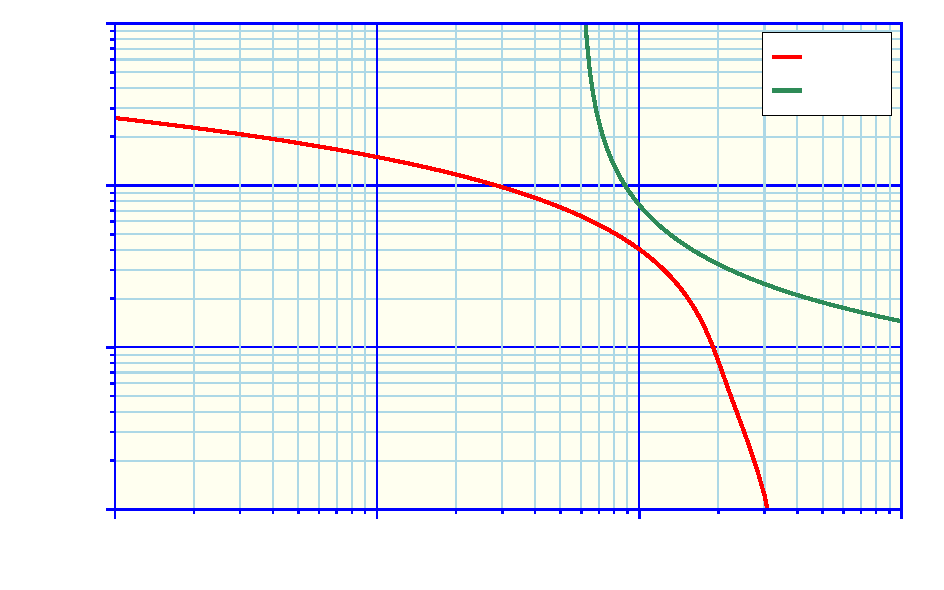
\includegraphics[width={453.00bp},height={283.00bp}]{Cap-Nornatives-Diverses-ProtInvIntVar}}%
    \gplfronttext
  \end{picture}%
\endgroup

	\end{center}
 	
 	A primera vista podria semblar que la protecció 51 no actua mai, ja que les dues corbes no s'entrecreuen. Aquesta deducció, però,  no és encertada pel fet que  no és estrictament correcte representar les dues corbes en un mateix gràfic, perquè tal com s'ha dit abans, la corba $t_{51}(I)$ representa temps d'actuació per a valors de $I$ constants, mentre que la corba $I\ped{a}(t)$ representa l'evolució d'un corrent variable en el temps.
 	
 	Per trobar el temps d'actuació ---si és que mai arriba a actuar--- de la corba $t_{51}(I)$, farem servir l'equació \eqref{eq:50-51-aprox}.  	Creem a continuació una taula per resoldre pas a pas l'equació esmentada; la taula té les columnes següents:
 	\begin{itemize}
 	 \item $i$. Indica el pas on som.
 	 \item $t_i$. Indica el temps del pas $i$; comença a \qty{0}{s}, i l'incrementem en intervals de  \qty{0,01}{s}.
 	 \item  $I\ped{a}(t_i)$. És el corrent de curtcircuit calculat a l'instant $t_i$, segons l'equació $I\ped{a}(t)$ d'aquest exemple.
 	 \item $t_{51}(I\ped{a}(t_i))$. És el temps d'actuació de la funció 51 quan circula un corrent constant $I\ped{a}(t_i)$, segons l'equació $t_{51}(I)$ d'aquest exemple.
 	 \item Àrea parcial. És el valor $\frac{1}{2} \left( \frac{1}{t_{51}(I(t_i))} + \frac{1}{t_{51}(I(t_{i-1}))} \right) (t_i - t_{i-1})$ de l'equació \eqref{eq:50-51-aprox}; representa, per tant, l'àrea entre dos intervals consecutius de temps.
 	 \item Àrea acumulada. És la suma acumulada de les àrees parcials, i, en conseqüència, representa l'àrea donada per l'equació \eqref{eq:50-51-aprox} entre $t_1$ i $t_i$.
    \end{itemize}
 	
 	
    \begin{center}
    	\centering
    	\begin{tabular}{S[table-format=2.0]S[table-format=1.2]
    	                S[table-format=5.3]S[table-format=1.4]
    	            	S[table-format=1.6]S[table-format=1.6]}
    	\toprule[1pt]
    	{$i$}  &  {$t_i\,/\,\unit{s}$}  &  {$I\ped{a}(t_i)\,/\,\unit{A}$}  & {$t_{51}(I\ped{a}(t_i))\,/\,\unit{s}$}  & {Àrea parcial}  & {Àrea acumulada} \\
    	\midrule
    	 1  &  0,00  &  36349,660  &  0,2213  &  {}        &  {}       \\
         2  &  0,01  &  30920,548  &  0,2422  &  0,043229  &  0,043229 \\
    	 3  &  0,02  &  27416,765  &  0,2607  &  0,039821  &  0,083050 \\
    	 4  &  0,03  &  25093,021  &  0,2762  &  0,037281  &  0,120331 \\
    	 5  &  0,04  &  23489,012  &  0,2891  &  0,035393  &  0,155724 \\
    	 6  &  0,05  &  22326,192  &  0,3000  &  0,033961  &  0,189685 \\
    	 7  &  0,06  &  21437,208  &  0,3092  &  0,032838  &  0,222524 \\
    	 8  &  0,07  &  20721,140  &  0,3174  &  0,031920  &  0,254444 \\
    	 9  &  0,08  &  20116,517  &  0,3250  &  0,031136  &  0,285580 \\
    	10  &  0,09  &  19585,434  &  0,3321  &  0,030440  &  0,316019 \\
    	11  &  0,10  &  19104,228  &  0,3391  &  0,029801  &  0,345821 \\
    	12  &  0,11  &  18657,956  &  0,3459  &  0,029201  &  0,375021 \\
    	13  &  0,12  &  18237,085  &  0,3528  &  0,028625  &  0,403646 \\
    	14  &  0,13  &  17835,465  &  0,3599  &  0,028066  &  0,431712 \\
    	15  &  0,14  &  17449,089  &  0,3670  &  0,027517  &  0,459229 \\
    	16  &  0,15  &  17075,311  &  0,3744  &  0,026975  &  0,486204 \\
    	17  &  0,16  &  16712,358  &  0,3821  &  0,026438  &  0,512643 \\
    	18  &  0,17  &  16359,017  &  0,3900  &  0,025905  &  0,538547 \\
    	19  &  0,18  &  16014,441  &  0,3983  &  0,025372  &  0,563920 \\
    	20  &  0,19  &  15678,017  &  0,4069  &  0,024842  &  0,588762 \\
    	21  &  0,20  &  15349,288  &  0,4159  &  0,024311  &  0,613073 \\
    	22  &  0,21  &  15027,900  &  0,4252  &  0,023782  &  0,636854 \\
    	23  &  0,22  &  14713,568  &  0,4350  &  0,023252  &  0,660106 \\
    	24  &  0,23  &  14406,053  &  0,4453  &  0,022722  &  0,682828 \\
    	25  &  0,24  &  14105,147  &  0,4561  &  0,022192  &  0,705020 \\
    	26  &  0,25  &  13810,667  &  0,4674  &  0,021662  &  0,726682 \\
    	27  &  0,26  &  13522,444  &  0,4792  &  0,021131  &  0,747813 \\
    	28  &  0,27  &  13240,324  &  0,4918  &  0,020600  &  0,768414 \\
    	29  &  0,28  &  12964,160  &  0,5050  &  0,020069  &  0,788483 \\
    	30  &  0,29  &  12693,813  &  0,5189  &  0,019537  &  0,808020 \\
    	31  &  0,30  &  12429,150  &  0,5336  &  0,019005  &  0,827026 \\
    	32  &  0,31  &  12170,044  &  0,5493  &  0,018473  &  0,845499 \\
    	33  &  0,32  &  11916,372  &  0,5658  &  0,017940  &  0,863438 \\
    	\midrule
    	\end{tabular}
	\end{center}
    	
    \begin{center}
	\centering
	\begin{tabular}{S[table-format=2.0]S[table-format=1.2]
			S[table-format=5.3]S[table-format=1.4]
			S[table-format=1.6]S[table-format=1.6]}
		\toprule[1pt]
		{$i$}  &  {$t_i\,/\,\unit{s}$}  &  {$I\ped{a}(t_i)\,/\,\unit{A}$}  & {$t_{51}(I\ped{a}(t_i))\,/\,\unit{s}$}  & {Àrea parcial}  & {Àrea acumulada} \\
		\midrule
		34  &  0,33  &  11668,014  &  0,5835  &  0,017406  &  0,880844 \\
		35  &  0,34  &  11424,855  &  0,6022  &  0,016872  &  0,897717 \\
		36  &  0,35  &  11186,783  &  0,6223  &  0,016338  &  0,914054 \\
		37  &  0,36  &  10953,688  &  0,6437  &  0,015803  &  0,929857 \\
		38  &  0,37  &  10725,463  &  0,6667  &  0,015267  &  0,945124 \\
		39  &  0,38  &  10502,006  &  0,6914  &  0,014731  &  0,959855 \\
		40  &  0,39  &  10283,214  &  0,7181  &  0,014195  &  0,974050 \\
		41  &  0,40  &  10068,989  &  0,7469  &  0,013657  &  0,987707 \\
		42  &  0,41  &   9859,235  &  0,7782  &  0,013120  &  1,000827 \\
		\bottomrule[1pt]
	\end{tabular}
\end{center}
    
Tal com es veu, entre $t = \qty{0,40}{s}$ i $t = \qty{0,41}{s}$, l'àrea acumulada arriba al valor 1. Això ens indica que la protecció 51 actuarà en aquest temps.

Si reféssim aquest exemple, canviant en l'equació $t_{51}(I)$ el valor multiplicatiu 0,6 per 0,8, veuríem que l'àrea acumulada no arriba mai a 1, sinó que es queda al voltant del valor 0,86; això ens indica que en aquest cas la protecció 51 no actuaria.

\end{exemple}	
	
	

\section{Grau de protecció IP} \label{sec:grau-IP}\index{IP} \index{grau de protecció} \index{CEI!60529-00@60529}

La codificació IP (\textit{International Protection Marking})  segons la
norma CEI 60529 \textit{Degrees of protection provided by enclosures (IP code)}, s'utilitza per descriure el grau de
protecció  proporcionat pels elements envoltants d'equips elèctrics, contra
l'entrada de cossos sòlids estranys i contra els efectes nocius
de l'aigua.

La codificació consisteix en les lletres «IP»
seguides per dues xifres, més una lletra addicional opcional, i una
lletra suplementària opcional; quan el grau de protecció
corresponent a una de les dues xifres no s'utilitzi, perquè no sigui
necessari o perquè no sigui conegut, es reemplaçarà la xifra en
qüestió per la lletra «X». Es defineix a continuació el
significat de les xifres i lletres que formen el codi IP:

\textbf{1a xifra}. Indica el grau de protecció a les persones contra els contactes amb
parts en tensió o amb peces en moviment, i el grau de protecció als equips contra l'entrada de cossos sòlids i pols. Els valors possibles són els següents:
\begin{list}{}
   {\setlength{\labelwidth}{10mm} \setlength{\leftmargin}{15mm} \setlength{\labelsep}{5mm}}
   \item[0] Sense cap protecció en particular.
   \item[1]Protecció contra l'entrada de cossos sòlids de diàmetre superior a \qty{50}{mm},
   com per exemple   contactes involuntaris de la mà.
   \item[2] Protecció contra l'entrada de cossos de diàmetre superior a \qty{12}{mm}, com per exemple
   contactes involuntaris dels dits de la mà.
   \item[3] Protecció contra l'entrada de cossos de diàmetre superior a \qty{2,5}{mm},
   com per exemple eines o cables.
   \item[4] Protecció contra l'entrada de cossos de diàmetre superior a \qty{1}{mm}.
   \item[5] Protecció contra la pols; se'n permet l'entrada allà on no sigui perjudicial.
   \item[6] Protecció total contra la pols.
\end{list}

\textbf{2a xifra}. Indica el grau de protecció dels equips contra
l'entrada d'aigua. Els valors possibles són els següents:
\begin{list}{}
   {\setlength{\labelwidth}{10mm} \setlength{\leftmargin}{15mm} \setlength{\labelsep}{5mm}}
   \item[0] Sense cap protecció en particular.
   \item[1] Protecció contra la caiguda vertical de gotes d'aigua.
   \item[2] Protecció contra la caiguda de gotes d'aigua fins a \ang{15} de la  vertical.
   \item[3] Protecció contra la caiguda de pluja fina ---polvoritzada--- fins a \ang{60} de la  vertical.
   \item[4] Protecció contra la caiguda d'aigua en totes les direccions.
   \item[5] Protecció contra aigua llançada a raig amb mànegues.
   \item[6] Protecció contra aigua llançada a raigs forts o per cops de mar.
   \item[7] Protecció contra la immersió temporal.
   \item[8] Protecció contra la immersió prolongada o a gran pressió.
\end{list}


\textbf{Lletra addicional opcional}. En alguns casos la protecció
proporcionada pels elements envoltants contra l'accés a les parts
perilloses és millor que la indicada per la primera xifra del codi.
En aquests casos es pot caracteritzar aquesta protecció amb una
lletra addicional, afegida després de les dues xifres; aquesta indicació és útil per a  envoltants que malgrat tenir obertures adequades per a la ventilació,  mantenen alhora el
grau requerit de protecció a les persones. Els valors possibles són
els següents:
\begin{list}{}
   {\setlength{\labelwidth}{10mm} \setlength{\leftmargin}{15mm} \setlength{\labelsep}{5mm}}
   \item[A] Els  cossos estranys de diàmetre superior a
   \qty{50}{mm}    poden entrar en l'element envoltant, però només d'una forma voluntària i deliberada.
   \item[B] Els  cossos estranys de diàmetre superior a \qty{12}{mm}
    poden entrar en l'element envoltant, però un dit de la mà no ha de poder entrar més de \qty{80}{mm}, i
    ha de quedar, doncs, a una distància    suficient de les parts perilloses.
   \item[C] Els  cossos estranys de diàmetre superior a \qty{2,5}{mm}
   poden entrar en l'element envoltant, però un filferro d'acer d'aquest diàmetre i \qty{100}{mm}
   de longitud ha de quedar a una distància suficient de les parts perilloses.
   \item[D] Els  cossos estranys de diàmetre superior a \qty{1}{mm}
   poden entrar en l'element envoltant, però un filferro d'acer d'aquest diàmetre i \qty{100}{mm}
   de longitud, ha de quedar a una distància suficient de les parts perilloses.
\end{list}

\textbf{Lletra suplementària opcional}. El codi IP accepta també algunes
lletres suplementàries al final, per tal d'afegir una informació concreta. Els valors
possibles són els següents:
\begin{list}{}
   {\setlength{\labelwidth}{10mm} \setlength{\leftmargin}{15mm} \setlength{\labelsep}{5mm}}
   \item[H] Material d'alta tensió.
   \item[M] En màquines rotatives indica que els assajos s'han realitzat amb el
    rotor girant.
   \item[S] En màquines rotatives indica que els assajos s'han dut a terme amb el
    rotor parat.
   \item[W] Protecció contra la intempèrie.
\end{list}


Algunes versions antigues del codi IP poden tenir una tercera xifra que indica la resistència a impactes mecànics, no obstant això, avui  dia la norma CEI 60529 ja no recull aquesta tercera xifra, i la resistència a impactes mecànics ve indicada pel codi IK (vegeu l'apartat següent). Aquesta tercera xifra donava el grau de resistència de l'element envoltant a una certa energia d'impacte:
\begin{list}{}
   {\setlength{\labelwidth}{10mm} \setlength{\leftmargin}{15mm} \setlength{\labelsep}{5mm}}
   \item[0] Cap resistència en particular a l'impacte.
   \item[1] Resisteix una energia d'impacte de \qty{0,225}{J}, equivalent a l'impacte d'una massa de \qty{150}{g} deixada anar des d'una altura de \qty{15}{cm}.
   \item[2] Resisteix una energia d'impacte de \qty{0,375}{J}, equivalent a l'impacte d'una massa de \qty{250}{g} deixada anar des d'una altura de \qty{15}{cm}.
   \item[3] Resisteix una energia d'impacte de \qty{0,5}{J}, equivalent a l'impacte d'una massa de \qty{250}{g} deixada anar des d'una altura de \qty{20}{cm}.
   \item[5] Resisteix una energia d'impacte de \qty{2}{J}, equivalent a l'impacte d'una massa de \qty{500}{g} deixada anar des d'una altura de \qty{40}{cm}.
   \item[7] Resisteix una energia d'impacte de \qty{6}{J}, equivalent a l'impacte d'una massa d'\qty{1,5}{kg} deixada anar des d'una altura de \qty{40}{cm}.
   \item[9]Resisteix una energia d'impacte de \qty{20}{J}, equivalent a l'impacte d'una massa de \qty{5}{kg} deixada anar des d'una altura de \qty{40}{cm}.
\end{list}

\section{Codi IK de resistència a impactes}\label{sec:codi-IK} \index{IK} \index{resistència a impactes} \index{CEI!62262-00@62262}

Actualment, el codi IK definit en la norma CEI 62262 \textit{Degrees of protection provided by enclosures for electrical equipment against external mechanical impacts (IK Code)}, és el que defineix la resistència d'un element  envoltant als impactes mecànics. Aquest codi és format per les lletres «IK» seguides d'un número de dues xifres, el qual indica el grau de resistència de l'element envoltant a una certa energia d'impacte:

\begin{list}{}
   {\setlength{\labelwidth}{10mm} \setlength{\leftmargin}{15mm} \setlength{\labelsep}{5mm}}
   \item[00] Cap resistència en particular a l'impacte.
   \item[01] Resisteix una energia d'impacte de \qty{0,15}{J}, equivalent a l'impacte d'una massa de \qty{200}{g} deixada anar des d'una altura de \qty{7,5}{cm}.
   \item[02] Resisteix una energia d'impacte de \qty{0,2}{J}, equivalent a l'impacte d'una massa de \qty{200}{g} deixada anar des d'una altura de \qty{10}{cm}.
   \item[03] Resisteix una energia d'impacte de \qty{0,35}{J}, equivalent a l'impacte d'una massa de \qty{200}{g} deixada anar des d'una altura de \qty{17,5}{cm}.
   \item[04] Resisteix una energia d'impacte de \qty{0,5}{J}, equivalent a l'impacte d'una massa de \qty{200}{g} deixada anar des d'una altura de \qty{25}{cm}.
   \item[05] Resisteix una energia d'impacte de \qty{0,7}{J}, equivalent a l'impacte d'una massa de \qty{200}{g} deixada anar des d'una altura de \qty{35}{cm}.
   \item[06]Resisteix una energia d'impacte d'\qty{1}{J}, equivalent a l'impacte d'una massa de \qty{500}{g} deixada anar des d'una altura de \qty{20}{cm}.
   \item[07]Resisteix una energia d'impacte de \qty{2}{J}, equivalent a l'impacte d'una massa de \qty{500}{g} deixada anar des d'una altura de \qty{40}{cm}.
   \item[08]Resisteix una energia d'impacte de \qty{5}{J}, equivalent a l'impacte d'una massa d'\qty{1,7}{kg} deixada anar des d'una altura de \qty{29,5}{cm}.
   \item[09]Resisteix una energia d'impacte de \qty{10}{J}, equivalent a l'impacte d'una massa de \qty{5}{kg} deixada anar des d'una altura de \qty{20}{cm}.
   \item[10]Resisteix una energia d'impacte de \qty{20}{J}, equivalent a l'impacte d'una massa de \qty{5}{kg} deixada anar des d'una altura de \qty{40}{cm}.
\end{list}



\section{Codi NEMA d'elements envoltants}
\index{codis NEMA d'elements envoltants} \index{NEMA!250}

La \textit{National Electrical Manufacturers Association} (NEMA)
codifica els elements envoltants en la norma NEMA 250 \textit{Enclosures for Electrical Equipment (1000 Volts Maximum)}, de manera similar al codi IP, segons el seu grau de protecció contra elements externs nocius. Podeu trobar més informació a l'adreça: \href{https://www.nema.org/standards/view/nema-250-enclosure-types}{https:/\!\!/www.nema.org/standards/view/nema-250-enclosure-types}.

Aquesta norma defineix els següents valors:

\begin{list}{}
   {\setlength{\labelwidth}{10mm} \setlength{\leftmargin}{15mm} \setlength{\labelsep}{5mm}}
   \item[1] Protecció contra la pols, però no de forma total, i contra les esquitxades suaus o indirectes; impedeix el contacte accidental amb els equips interns. S'utilitza en interiors, en condicions atmosfèriques normals.
   \item[2] Com el tipus 1, i a més ofereix protecció total contra el degoteig.
   \item[3] Protecció contra la pols, la pluja, l'aiguaneu i la neu; impedeix el contacte accidental amb els equips interns. S'utilitza en interiors o exteriors i pot suportar la formació de gel al seu damunt.
   \item[3R] Com el tipus 3, però sense protecció contra la pols.
   \item[3S] Com el tipus 3, i a més els mecanismes externs han de ser operables quan s'hi dipositi gel.
    \item[4] Protecció contra la pols, la pluja, l'aiguaneu, la neu, les esquitxades i els raigs d'aigua directes; impedeix el contacte accidental amb els equips interns. S'utilitza en interiors o exteriors i pot suportar la formació de gel al seu damunt.
   \item[4X] Com el tipus 4, i a més ofereix protecció contra la corrosió.
   \item[5] Protecció contra la pols i contra les esquitxades suaus o indirectes; impedeix el contacte accidental amb els equips interns. S'utilitza en interiors.
   \item[6] Protecció contra els raigs d'aigua directes i contra l'entrada d'aigua en ser submergit un temps curt; impedeix el contacte accidental amb els equips interns. S'utilitza en interiors o exteriors i pot suportar la formació de gel al seu damunt.
   \item[6P] Com el tipus 6, però protegit contra l'entrada d'aigua en ser submergit durant un temps més llarg.
   \item[7] S'utilitza en interiors, en ambients perillosos definits per la norma NEC com a classe I, grups A, B, C o D.
   \item[8] Com el tipus 7, però d'ús interior i exterior.
   \item[9] S'utilitza en interiors i exteriors, en ambients perillosos definits per la norma NEC com a classe II, grups E, F o G.
   \item[10] Compleix els requisits de la \textit{Mine Safety and Health Administration 30 CFR part 18}.
   \item[11] Protecció contra l'efecte corrosiu de líquids i gasos.
   \item[12] Protecció contra la pols en suspensió i contra les esquitxades suaus o indirectes; impedeix el contacte accidental amb els equips interns. S'utilitza en interiors.
   \item[12K] Com el tipus 12, però l'element envoltant pot tenir obertures.
   \item[13] Protecció contra la pols en suspensió i contra les esquitxades o ruixats d'aigua, oli o líquids no corrosius; impedeix el contacte accidental amb els equips interns. S'utilitza en interiors.
\end{list}



La taula \vref{taula:nema-IP} es pot utilitzar per trobar el codi IP equivalent a un codi NEMA donat; no ha d'utilitzar-se per a la conversió contrària.

\begin{center}
   \captionof{table}{Conversió de codis NEMA a codis IP}\label{taula:nema-IP}
   \begin{tabular}{cc}
   \toprule[1pt]
   Codi NEMA & Codi IP equivalent \\
   \midrule
   1 & IP10 \\
   2 & IP11 \\
   3 & IP54 \\
   3R & IP14 \\
   3S & IP54 \\
   4 i 4X & IP56 \\
   5 & IP52 \\
   6 i 6P & IP67\\
   12 i 12K & IP52 \\
   13 & IP54 \\
   \bottomrule[1pt]
   \end{tabular}
\end{center}


\section{Norma CEI 60947-2  d'interruptors automàtics  de baixa tensió}


Es donen a continuació algunes definicions incloses en la norma CEI 60947-2 \textit{Low-voltage switchgear and controlgear --- Circuit-breakers}, referents als interruptors automàtics de baixa tensió, és a dir, tensions que no passin de \qty{1000}{V} en corrent altern, o de \qty{1500}{V} en corrent continu.\index{CEI!60947-2}

Aquesta norma defineix un interruptor automàtic de la manera següent: Aparell mecànic de connexió capaç d'establir, de suportar i d'interrompre el corrent en les condicions normals d'un circuit, així com d'establir, de suportar durant un temps especificat i  d'interrompre el corrent en les condicions anormals especificades d'un circuit, com per exemple el que apareix durant un curtcircuit.

Un interruptor automàtic es diu que és limitador de corrent, quan el seu temps d'obertura és particularment breu, per tal d'evitar que el corrent que s'origina en un curtcircuit arribi al seu valor màxim.

Quan tenim dos  dispositius de protecció ---interruptors automàtics, fusibles, etc.--- en sèrie, la selectivitat es diu que és total si per a qualsevol valor del corrent, el dispositiu situat aigües avall obre sempre abans que ho faci el dispositiu situat aigües amunt. La selectivitat es diu que és parcial, si l'obertura del dispositiu situat aigües avall, abans que ho faci el dispositiu situat aigües amunt, només està garantida fins a un cert valor del corrent $I\ped{s}$, anomenat corrent límit de selectivitat; $I\ped{s}$ correspon al punt d'intersecció de les característiques corrent-temps dels dos dispositius de protecció. En el cas d'interruptors automàtics es defineixen dues categories d'ús:\index{Is@$I\ped{s}$}
 \begin{list}{}
   {\setlength{\labelwidth}{10mm} \setlength{\leftmargin}{15mm} \setlength{\labelsep}{5mm}}
   \item[A] Interruptors automàtics que no estan específicament preparats per ser selectius en condicions de curtcircuit amb altres dispositius de protecció situats en sèrie  aigües avall.
   \item[B] Interruptors automàtics específicament concebuts per ser selectius en condicions de curtcircuit amb altres dispositius de protecció situats en sèrie  aigües avall. Aquests interruptors han d'especificar el seu corrent admissible de curta durada $I\ped{cw}$.
\end{list}

Es relacionen a continuació les definicions de diversos paràmetres dels interruptors automàtics; es dona entre parèntesis el nom equivalent en anglès:
\begin{list}{}
   {\setlength{\labelwidth}{10mm} \setlength{\leftmargin}{15mm} \setlength{\labelsep}{5mm}}
   \item[$U\ped{e}$] Tensió nominal d'operació (\textit{rated operational voltage}).\index{Ue@$U\ped{e}$}
   \item[$U\ped{i}$] Tensió nominal d'aïllament (\textit{rated insulation voltage}). És el valor de tensió utilitzat en els assajos dielèctrics de l'interruptor;  el valor més elevat de $U\ped{e}$ no pot ser mai superior a $U\ped{i}$.\index{Ui@$U\ped{i}$}
    \item[$U\ped{imp}$] Tensió nominal d'impuls suportada (\textit{rated impulse withstand voltage}). És el valor de pic d'una tensió d'impuls, de forma i polaritat predeterminades, que l'interruptor pot suportar.\index{Uimp@$U\ped{imp}$}
   \item[$I\ped{th}$] Corrent tèrmic convencional a l'aire lliure (\textit{conventional free-air thermal current}).  És la  màxima intensitat de corrent a utilitzar en els assajos d'escalfament de l'interruptor sense cap element envoltant, a l'aire lliure.\index{Ith@$I\ped{th}$}
   \item[$I\ped{the}$] Corrent tèrmic convencional dins d'un element envoltant (\textit{conventional enclosed thermal current}).  És la màxima intensitat de corrent a utilitzar en els assajos d'escalfament de l'interruptor, quan està situat dins d'un element envoltant especificat.\index{Ithe@$I\ped{the}$}
    \item[$I\ped{u}$] Corrent nominal ininterromput (\textit{rated uninterrupted current}).  És la intensitat  de corrent, fixada pel fabricant, que l'interruptor pot suportar de manera ininterrompuda.\index{Iu@$I\ped{u}$}
    \item[$I\ped{n}$] Corrent nominal (\textit{rated current}).  En els interruptors automàtics és equivalent a $I\ped{u}$ i té el mateix valor que $I\ped{th}$.\index{In@$I\ped{n}$}
    \item[$I\ped{cu}$] Poder nominal de tall últim en curtcircuit (\textit{rated ultimate  short-circuit breaking capacity}). És la capacitat que té l'interruptor d'obrir en curtcircuit a la tensió nominal d'operació, en un cicle d'assaig del tipus O-t-CO (obrir, tancar i obrir); s'expressa pel valor eficaç simètric del corrent esperat, en kA. Després de l'assaig no es requereix que l'interruptor pugui suportar en règim continu el seu corrent nominal.\index{Icu@$I\ped{cu}$}
    \item[$I\ped{cs}$] Poder nominal de tall de servei en curtcircuit (\textit{rated service  short-circuit breaking capacity}). És la capacitat que té l'interruptor d'obrir en curtcircuit a la tensió nominal d'operació, en un cicle d'assaig del tipus O-t-CO-t-CO (obrir, tancar i obrir, tancar i obrir); s'expressa pel valor  del corrent esperat, en kA, corresponent a un dels percentatges de $I\ped{cu}$ especificats en la taula \vref{taula:IcsIcu}, arrodonit al valor enter més pròxim. Després de l'assaig l'interruptor cal que pugui suportar en règim continu  el seu corrent nominal.\index{Ics@$I\ped{cs}$}

        \begin{center}
           \captionof{table}{Valors de I$_\text{cs}$ segons la categoria d'ús} \label{taula:IcsIcu}
           \begin{tabular}{cc}
           \toprule[1pt]
           Categoria d'ús &  Valors possibles de $I\ped{cs}$ \\
           \midrule
           A & $\qtylist[list-units = brackets]{25;50;75;100}{\percent} I\ped{cu}$ \\
           B & $\qtylist[list-units = brackets]{50;75;100}{\percent} I\ped{cu}$  \\
           \bottomrule[1pt]
           \end{tabular}
         \end{center}
    \item[$I\ped{cm}$] Poder nominal de tancament en curtcircuit (\textit{rated short-circuit making capacity}). És la capacitat que té l'interruptor de tancar en curtcircuit a la tensió nominal d'operació, per a un factor de potència especificat en corrent altern, o per a una constant de temps especificada en corrent continu; s'expressa pel valor màxim de pic del corrent esperat. En el cas de corrent altern ha de complir-se: $I\ped{cm} \geq n I\ped{cu}$; els valors possibles del paràmetre $n$ poden veure's en la taula \vref{taula:IcmIcu}.\index{Icm@$I\ped{cm}$}

      \begin{center}
           \captionof{table}{Valors n que relacionen I$_\text{cm}$ amb I$_\text{cu}$} \label{taula:IcmIcu}
           \begin{tabular}{r<{\hspace{-0.7em}}c<{\hspace{-0.7em}}rSS}
           \toprule[1pt]
            & $I\ped{cu}$  & &  {Factor de potència} & {$n$} \\
           \midrule
           \qty{4,5}{kA} & $\leq I\ped{cu} \leq$ & \qty{6}{kA} & 0,7  & 1,5   \\
           \qty{6}{kA} & $< I\ped{cu} \leq$ & \qty{10}{kA}     & 0,5  & 1,7   \\
           \qty{10}{kA} & $< I\ped{cu} \leq$ & \qty{20}{kA}    & 0,30  & 2,0   \\
           \qty{20}{kA} & $< I\ped{cu} \leq$ & \qty{50}{kA}    & 0,25 & 2,1   \\
           &  \phantom{00}$I\ped{cu} >$ & \qty{50}{kA}     & 0,2  & 2,2   \\
           \bottomrule[1pt]
           \end{tabular}
        \end{center}
    \item[$I\ped{cw}$] Corrent nominal de curta durada admissible (\textit{rated short-time withstand current}). És el corrent que pot suportar un interruptor de categoria d'ús B durant un temps convencional, sense danyar-se i sense que se n'alterin les característiques, obtenint-se així la possibilitat de ser selectiu amb altres dispositius de protecció situats en sèrie  aigües avall; s'expressa pel valor eficaç simètric del corrent esperat, en kA. El temps mínim que ha de suportar el corrent és \qty{0,05}{s}, i els valors preferits són: \qtylist{0,05;0,1;0,25;0,5;1}{s}. El valor mínim que ha de tenir $I\ped{cw}$ pot veure's en la taula \vref{taula:InIcw}. \index{Icw@$I\ped{cw}$}

        \begin{center}
           \captionof{table}{Valors de I$_\text{cw}$ en funció de I$_\text{n}$} \label{taula:InIcw}
           \begin{tabular}{cc}
           \toprule[1pt]
           $I\ped{n}$ &  Valor mínim de $I\ped{cw}$ \\
           \midrule
           $I\ped{n} \leq \qty{2500}{A}$  & màxim entre $12  I\ped{n}$ i \qty{15}{kA}  \\
           $I\ped{n} > \qty{2500}{A}$  & \qty{30}{kA}   \\
           \bottomrule[1pt]
           \end{tabular}
        \end{center}
\end{list}


\section{Àmbit d'aplicació de diverses Normes CEI}\index{CEI}\label{sec:normes_IEC}

Es relacionen a continuació diverses normes de la CEI \textit{Commission électrotechnique internationale} (o en anglès: IEC \textit{International Electrotechnical Commission}), agrupades pel seu àmbit d'aplicació. Podeu trobar el llistat complet de les normes CEI a l'adreça: \href{https://www.iec.ch/homepage}{https:/\!\!/www.iec.ch/homepage}. S'indica també alguna norma ISO \textit{International Organization for Standardization}, de la sèrie 80000.

\subsection*{Aparellatge de baixa tensió}
\begin{description}
	
	\item [\hspace{5mm}CEI 60947-1.] \textit{Low-voltage switchgear and controlgear --- Part 1: General rules}.\index{CEI!60947-1}
	\item [\hspace{5mm}CEI 60947-2.] \textit{Low-voltage switchgear and controlgear --- Part 2: Circuit-breakers}.\index{CEI!60947-2}
	\item [\hspace{5mm}CEI 60947-3.] \textit{Low-voltage switchgear and controlgear --- Part 3: Switches, disconnectors, switch-dis\-con\-nec\-tors and fuse-combination units}.\index{CEI!60947-3}
	\item [\hspace{5mm}CEI 60947-4-1.] \textit{Low-voltage switchgear and controlgear --- Part 4-1: Contactors and motor starters ---  Electromechanical contactors and motor starters}.\index{CEI!60947-4-1}
	\item [\hspace{5mm}CEI 60947-4-2.] \textit{Low-voltage switchgear and controlgear --- Part 4-2: Contactors and motor starters ---  A.C. Semiconductor motor controllers and starters}.\index{CEI!60947-4-2}
	\item [\hspace{5mm}CEI 60947-4-3.] \textit{Low-voltage switchgear and controlgear --- Part 4-3: Contactors and motor starters ---  A.C. semiconductor controllers and contactors for non-motor loads}.\index{CEI!60947-4-3}
\end{description}



\subsection*{Aparellatge d'alta tensió}
\begin{description}
    \item [\hspace{5mm}CEI 62271-1.] \textit{High-voltage switchgear and controlgear --- Part 1: Common specifications}.\index{CEI!62271-1}
    \item [\hspace{5mm}CEI 62271-100.] \textit{High-voltage switchgear and controlgear --- Part 100: Alternating current circuit-breakers}.\index{CEI!62271-100}
    \item [\hspace{5mm}CEI 62271-102.] \textit{High-voltage switchgear and controlgear --- Part 102: Alternating current disconnectors and earthing switches}.\index{CEI!62271-102}
    \item [\hspace{5mm}CEI 62271-103.] \textit{High-voltage switchgear and controlgear --- Part 103: Switches for rated voltages above 1 kV up to and including 52 kV}.\index{CEI!62271-103}
\end{description}


\subsection*{Aparells de mesura}
\begin{description}
	\item [\hspace{5mm}CEI 60051-1.] \textit{Direct acting indicating analogue electrical measuring instruments and their accessories --- Part 1:  Definitions and general requirements common to all parts}.\index{CEI!60051-1}
	\item [\hspace{5mm}CEI 60051-2.] \textit{Direct acting indicating analogue electrical measuring instruments and their accessories --- Part 2:  Special requirements for ammeters and voltmeters}.\index{CEI!60051-2}
	\item [\hspace{5mm}CEI 60051-3.] \textit{Direct acting indicating analogue electrical measuring instruments and their accessories --- Part 3: Special requirements for wattmeters and varmeters}.\index{CEI!60051-3}
	\item [\hspace{5mm}CEI 60051-4.] \textit{Direct acting indicating analogue electrical measuring instruments and their accessories  --- Part 4:  Special requirements for frequency meters}.\index{CEI!60051-4}
	\item [\hspace{5mm}CEI 60051-5.] \textit{Direct acting indicating analogue electrical measuring instruments and their accessories --- Part 5:  Special requirements for phase meters, power factor meters and synchroscopes}.\index{CEI!60051-5}
	\item [\hspace{5mm}CEI 60051-6.] \textit{Direct acting indicating analogue electrical measuring instruments and their accessories --- Part 6:  Special requirements for ohmmeters (impedance meters) and conductance meters}.\index{CEI!60051-6}
	\item [\hspace{5mm}CEI 60051-7.] \textit{Direct acting indicating analogue electrical measuring instruments and their accessories --- Part 7:  Special requirements for multi-function instruments}.\index{CEI!60051-7}
	\item [\hspace{5mm}CEI 60051-8.] \textit{Direct acting indicating analogue electrical measuring instruments and their accessories --- Part 8:  Special requirements for accessories}.\index{CEI!60051-8}
	\item [\hspace{5mm}CEI 60051-9.] \textit{Direct acting indicating analogue electrical measuring instruments and their accessories --- Part 9:  Recommended test methods}.\index{CEI!60051-9}
\end{description}


\subsection*{Coordinació d'aïllaments}
\begin{description}
    \item [\hspace{5mm}CEI 60071-1.] \textit{Insulation co-ordination --- Part 1: Definitions, principles and rules}.\index{CEI!60071-1}
    \item [\hspace{5mm}CEI 60071-2.] \textit{Insulation co-ordination --- Part 2: Application guide}.\index{CEI!60071-2}
    \item [\hspace{5mm}CEI 60071-3.] \textit{Insulation co-ordination --- Part 3: Phase to phase insulation coordination. Principles, rules and application guide}.\index{CEI!60071-3}
    \item [\hspace{5mm}CEI 60071-4.] \textit{Insulation co-ordination --- Part 4: Computational guide to insulation co-ordination and modelling of electrical networks}.\index{CEI!60071-4}
    \item [\hspace{5mm}CEI 60071-5.] \textit{Insulation co-ordination --- Part 5: Procedures for high-voltage direct current (HVDC) converter stations}.\index{CEI!60071-5}
\end{description}


\subsection*{Curtcircuits}
\begin{description}
    \item [\hspace{5mm}CEI 60909-0.] \textit{Short-circuit currents in three-phase a.c. systems --- Part 0: Calculation of currents}.\index{CEI!60909-0}
    \item [\hspace{5mm}CEI 60909-1.] \textit{Short-circuit currents in three-phase a.c. systems --- Part 1:  Factors for the calculation of short-circuit currents according to IEC 60909-0}.\index{CEI!60909-1}
    \item [\hspace{5mm}CEI 60909-2.] \textit{Short-circuit currents in three-phase a.c. systems --- Part 2:  Data of electrical equipment for short-circuit current calculations}.\index{CEI!60909-2}
    \item [\hspace{5mm}CEI 60909-3.] \textit{Short-circuit currents in three-phase a.c. systems --- Part 3: Currents during two separate simultaneous line-to-earth short circuits and partial short-circuit currents flowing through earth}.\index{CEI!60909-3}
    \item [\hspace{5mm}CEI 60909-4.] \textit{Short-circuit currents in three-phase a.c. systems --- Part 4: Examples for the calculation of short-circuit currents}.\index{CEI!60909-4}
\end{description}

\subsection*{Envoltants d'equips elèctrics}
\begin{description}
	\item [\hspace{5mm}CEI 60529.] \textit{Degrees of protection provided by enclosures (IP code)}.\index{CEI!60529-00@60529}
	\item [\hspace{5mm}CEI 62262.] \textit{Degrees of protection provided by enclosures for electrical equipment against external mechanical impacts (IK Code)}.\index{CEI!62262-00@62262}
\end{description}

\subsection*{Fusibles de baixa tensió}
\begin{description}
    \item [\hspace{5mm}CEI 60269-1.] \textit{Low-voltage fuses --- Part 1: General requirements}.\index{CEI!60269-1}
    \item [\hspace{5mm}CEI 60269-2.] \textit{Low-voltage fuses --- Part 2: Supplementary requirements for fuses for use by authorized persons
          (fuses mainly for industrial application) ---  Examples of standardized systems of fuses A to J}.\index{CEI!60269-2}
\end{description}

\subsection*{Motors}
\begin{description}
    \item [\hspace{5mm}CEI 60034-1.] \textit{Rotating electrical machines --- Part 1: Rating and performance}.\index{CEI!60034-01@60034-1}
    \item [\hspace{5mm}CEI 60034-2.] \textit{Rotating electrical machines --- Part 2: Methods for determining losses and
efficiency of rotating electrical machinery from tests (excluding machines for traction vehicles}).\index{CEI!60034-02@60034-2}
    \item [\hspace{5mm}CEI 60034-5.] \textit{Rotating electrical machines --- Part 5: Degrees of protection provided by the
integral design of rotating electrical machines (IP code) ---  Classification}.\index{CEI!60034-05@60034-5}
    \item [\hspace{5mm}CEI 60034-6.] \textit{Rotating electrical machines --- Part 6: Methods of cooling (IC code)}.\index{CEI!60034-06@60034-6}
    \item [\hspace{5mm}CEI 60034-7.] \textit{Rotating electrical machines --- Part 7: Classification of types of construction, mounting arrangements and terminal box position (IM Code)}.\index{CEI!60034-07@60034-7}
    \item [\hspace{5mm}CEI 60034-8.] \textit{Rotating electrical machines --- Part 8: Terminal markings and direction of
rotation}.\index{CEI!60034-08@60034-8}
    \item [\hspace{5mm}CEI 60034-12.] \textit{Rotating electrical machines --- Part 12: Starting performance of single-speed
three-phase cage induction motors}.\index{CEI!60034-12@60034-12}
    \item [\hspace{5mm}CEI 60034-15.] \textit{Rotating electrical machines --- Part 15: Impulse voltage withstand levels of
rotating a.c. machines with form-wound stator coils}.\index{CEI!60034-15@60034-15}
    \item [\hspace{5mm}CEI 60034-17.] \textit{Rotating electrical machines --- Part 17: Cage induction motors when fed from
converters --- Application guide}.\index{CEI!60034-17@60034-17}
    \item [\hspace{5mm}CEI 60034-18.] \textit{Rotating electrical machines --- Part 18: Functional evaluation of insulating
systems}.\index{CEI!60034-18@60034-18}
\end{description}

\subsection*{Proteccions elèctriques}
\begin{description}
    \item [\hspace{5mm}CEI 60255-1.] \textit{Measuring relays and protection equipment --- Part 1: Common requirements}.\index{CEI!60255-001@60255-1}
    \item [\hspace{5mm}CEI 60255-12.] \textit{Electrical relays --- Part 12: Directional relays and power relays with two input energizing quantities}.\index{CEI!60255-012@60255-12}
    \item [\hspace{5mm}CEI 60255-21.] \textit{Electrical relays --- Part 21: Vibration, shock, bump and seismic tests on measuring relays and protection equipment}.\index{CEI!60255-021@60255-21}
    \item [\hspace{5mm}CEI 60255-24.] \textit{Measuring relays and protection equipment --- Part 24: Common format for transient data exchange (COMTRADE) for power systems}.\index{CEI!60255-024@60255-24}
    \item [\hspace{5mm}CEI 60255-26.] \textit{Measuring relays and protection equipment --- Part 26: Electromagnetic compatibility requirements}.\index{CEI!60255-026@60255-26}
    \item [\hspace{5mm}CEI 60255-27.] \textit{Measuring relays and protection equipment --- Part 27: Product safety requirements}.\index{CEI!60255-027@60255-27}
    \item [\hspace{5mm}CEI 60255-118.] \textit{Measuring relays and protection equipment --- Part 118: Synchrophasor for power systems}.\index{CEI!60255-118}
    \item [\hspace{5mm}CEI 60255-121.] \textit{Measuring relays and protection equipment --- Part 121: Functional requirements for distance protection}.\index{CEI!60255-121}
    \item [\hspace{5mm}CEI 60255-127.] \textit{Measuring relays and protection equipment --- Part 127: Functional requirements for over/under voltage protection}.\index{CEI!60255-127}
    \item [\hspace{5mm}CEI 60255-149.] \textit{Measuring relays and protection equipment --- Part 149:  Functional requirements for thermal electrical relays}.\index{CEI!60255-149}
    \item [\hspace{5mm}CEI 60255-151.] \textit{Measuring relays and protection equipment --- Part 151:  Functional requirements for over/under current protection}.\index{CEI!60255-151}
    \item [\hspace{5mm}CEI 60255-181.] \textit{Measuring relays and protection equipment --- Part 181: Functional requirements for frequency protection}.\index{CEI!60255-181}   
\end{description}

\subsection*{Quadres elèctrics de baixa tensió}
\begin{description}
    \item [\hspace{5mm}CEI 61439-0.] \textit{Low-voltage switchgear and controlgear assemblies --- Part 0: Guidance to specifying assemblies}.\index{CEI!61439-0}
    \item [\hspace{5mm}CEI 61439-1.] \textit{Low-voltage switchgear and controlgear assemblies --- Part 1: General rules}.\index{CEI!61439-1}
    \item [\hspace{5mm}CEI 61439-2.] \textit{Low-voltage switchgear and controlgear assemblies --- Part 2: Power switchgear and controlgear assemblies}.\index{CEI!61439-2}
    \item [\hspace{5mm}CEI 61439-3.] \textit{Low-voltage switchgear and controlgear assemblies --- Part 3: Distribution boards intended to be operated by ordinary persons (DBO)}.\index{CEI!61439-3}
    \item [\hspace{5mm}CEI 61439-4.] \textit{Low-voltage switchgear and controlgear assemblies --- Part 4: Particular requirements for assemblies for construction sites (ACS)}.\index{CEI!61439-4}
    \item [\hspace{5mm}CEI 61439-5.] \textit{Low-voltage switchgear and controlgear assemblies --- Part 5: Assemblies for power distribution in public networks}.\index{CEI!61439-5}
    \item [\hspace{5mm}CEI 61439-6.] \textit{Low-voltage switchgear and controlgear assemblies --- Part 6: Busbar trunking systems (bus\-ways)}.\index{CEI!61439-6}
    \item [\hspace{5mm}CEI 61439-7.] \textit{Low-voltage switchgear and controlgear assemblies --- Part 7: Assemblies for specific applications such as marinas, camping sites, market squares, electric vehicles charging stations}.\index{CEI!61439-7}
\end{description}

\subsection*{Representació i simbologia}
\begin{description}
    \item [\hspace{5mm}CEI 60050.] \textit{International Electrotechnical Vocabulary}. \index{CEI!60050-00@60050}
    \item [\hspace{5mm}CEI 60617-1.] \textit{Graphical symbols for diagrams --- Part 1: General information, general index. Cross-reference tables}.\index{CEI!60617-01@60617-1}
    \item [\hspace{5mm}CEI 60617-2.] \textit{Graphical symbols for diagrams --- Part 2: Symbol elements, qualifying symbols and other symbols having general application}.\index{CEI!60617-02@60617-2}
    \item [\hspace{5mm}CEI 60617-3.] \textit{Graphical symbols for diagrams --- Part 3: Conductors and connecting devices}.\index{CEI!60617-03@60617-3}
    \item [\hspace{5mm}CEI 60617-4.] \textit{Graphical symbols for diagrams --- Part 4: Basic passive components}.\index{CEI!60617-04@60617-4}
    \item [\hspace{5mm}CEI 60617-5.] \textit{Graphical symbols for diagrams --- Part 5: Semiconductors and electron tubes}.\index{CEI!60617-05@60617-5}
    \item [\hspace{5mm}CEI 60617-6.] \textit{Graphical symbols for diagrams --- Part 6: Production and conversion of electrical energy}.\index{CEI!60617-06@60617-6}
    \item [\hspace{5mm}CEI 60617-7.] \textit{Graphical symbols for diagrams --- Part 7: Switchgear, controlgear and protective devices}.\index{CEI!60617-07@60617-7}
    \item [\hspace{5mm}CEI 60617-8.] \textit{Graphical symbols for diagrams --- Part 8: Measuring instruments, lamps and signalling devices}.\index{CEI!60617-08@60617-8}
    \item [\hspace{5mm}CEI 60617-9.] \textit{Graphical symbols for diagrams --- Part 9: Telecommunications: switching and peripheral equipment}.\index{CEI!60617-09@60617-9}
    \item [\hspace{5mm}CEI 60617-10.] \textit{Graphical symbols for diagrams --- Part 10: Telecommunications: transmission}.\index{CEI!60617-10}
    \item [\hspace{5mm}CEI 60617-11.] \textit{Graphical symbols for diagrams --- Part 11: Architectural and topographical installation plans and diagrams}.\index{CEI!60617-11}
    \item [\hspace{5mm}CEI 60617-12.] \textit{Graphical symbols for diagrams --- Part 12: Binary logic elements}.\index{CEI!60617-12}
    \item [\hspace{5mm}CEI 60617-13.] \textit{Graphical symbols for diagrams --- Part 13: Analogue elements}.\index{CEI!60617-13}
    \item [\hspace{5mm}ISO 80000-1.] \textit{Quantities and units --- Part 1: General}.\index{ISO!80000-01@80000-1}
    \item [\hspace{5mm}ISO 80000-2.] \textit{Quantities and units --- Part 2: Mathematics}.\index{ISO!80000-02@80000-2}
    \item [\hspace{5mm}ISO 80000-3.] \textit{Quantities and units --- Part 3: Space and time}. \index{ISO!80000-03@80000-3}
    \item [\hspace{5mm}ISO 80000-4.] \textit{Quantities and units --- Part 4: Mechanics}.\index{ISO!80000-04@80000-4}
    \item [\hspace{5mm}ISO 80000-5.] \textit{Quantities and units --- Part 5: Thermodynamics}.\index{ISO!80000-05@80000-5}
    \item [\hspace{5mm}CEI 80000-6.] \textit{Quantities and units --- Part 6: Electromagnetism}.\index{CEI!80000-06@80000-6}
    \item [\hspace{5mm}ISO 80000-7.] \textit{Quantities and units --- Part 7: Light and radiation}.\index{ISO!80000-07@80000-7}
    \item [\hspace{5mm}ISO 80000-8.] \textit{Quantities and units --- Part 8: Acoustics}.\index{ISO!80000-08@80000-8}
	\item [\hspace{5mm}ISO 80000-9.] \textit{Quantities and units --- Part 9: Physical chemistry and molecular physics}.\index{ISO!80000-09@80000-9}
	\item [\hspace{5mm}ISO 80000-10.] \textit{Quantities and units --- Part 10: Atomic and nuclear physics}.\index{ISO!80000-10}
	\item [\hspace{5mm}ISO 80000-11.] \textit{Quantities and units --- Part 11: Characteristic numbers}.\index{ISO!80000-11}
	\item [\hspace{5mm}ISO 80000-12.] \textit{Quantities and units --- Part 12: Condensed matter physics}.\index{ISO!80000-12}
	\item [\hspace{5mm}CEI 80000-13.] \textit{Quantities and units --- Part 13: Information science and technology}.\index{CEI!80000-13}
	\item [\hspace{5mm}CEI 80000-14.] \textit{Quantities and units --- Part 14: Telebiometrics related to human physiology}.\index{CEI!80000-14}
	\item [\hspace{5mm}CEI 80000-15.] \textit{Quantities and units --- Part 15: Logarithmic and related quantities}.\index{CEI!80000-15}
	\item [\hspace{5mm}CEI 80000-16.] \textit{Quantities and units --- Part 16: Printing and writing rules}.\index{CEI!80000-16}
	\item [\hspace{5mm}CEI 80000-17.] \textit{Quantities and units --- Part 17: Time dependency}.\index{CEI!80000-17}    
\end{description}

\subsection*{Resistències i condensadors} \index{resistències}\index{condensadors}
\begin{description}
	\item [\hspace{5mm}CEI 60062.] \textit{Marking codes for resistors and capacitors}.\index{CEI!60062-00@60062}	
	\item [\hspace{5mm}CEI 60063.] \textit{Preferred number series for resistors and capacitors}.\index{CEI!60063-00@60063}
\end{description}

\subsection*{Termoparells} \index{termoparells}
\begin{description}
    \item [\hspace{5mm}CEI 60584-1.] \textit{Thermocouples --- Part 1: Reference tables}.\index{CEI!60584-1}
    \item [\hspace{5mm}CEI 60584-2.] \textit{Thermocouples --- Part 2: Tolerances}.\index{CEI!60584-2}
    \item [\hspace{5mm}CEI 60584-3.] \textit{Thermocouples --- Part 3: Extension and compensating cables --- Tolerances and identification system}.\index{CEI!60584-3}
\end{description}


\subsection*{Transformadors de mesura i protecció}
\begin{description}
    \item [\hspace{5mm}CEI 60044-1.] \textit{Instrument transformers --- Part 1: Current transformers}.\index{CEI!60044-1}
    \item [\hspace{5mm}CEI 60044-2.] \textit{Instrument transformers --- Part 2: Inductive voltage transformers}.\index{CEI!60044-2}
    \item [\hspace{5mm}CEI 60044-3.] \textit{Instrument transformers --- Part 3: Combined transformers}.\index{CEI!60044-3}
    \item [\hspace{5mm}CEI 60044-4.] \textit{Instrument transformers --- Part 4: Measurement of partial discharges}.\index{CEI!60044-4}
    \item [\hspace{5mm}CEI 60044-5.] \textit{Instrument transformers --- Part 5: Capacitor voltage transformers}.\index{CEI!60044-5}
\end{description}


\subsection*{Transformadors de potència}
\begin{description}
    \item [\hspace{5mm}CEI 60076-1.] \textit{Power transformers --- Part 1: General}.\index{CEI!60076-01@60076-1}
    \item [\hspace{5mm}CEI 60076-2.] \textit{Power transformers --- Part 2: Temperature rise}.\index{CEI!60076-02@60076-2}
    \item [\hspace{5mm}CEI 60076-3.] \textit{Power transformers --- Part 3: Insulation levels, dielectric tests and external clearances in air}.\index{CEI!60076-03@60076-3}
    \item [\hspace{5mm}CEI 60076-4.] \textit{Power transformers --- Part 4: Guide to the lightning impulse and switching impulse testing --- Power transformers and reactors}.\index{CEI!60076-04@60076-4}
    \item [\hspace{5mm}CEI 60076-5.] \textit{Power transformers --- Part 5: Ability to withstand short circuit}.\index{CEI!60076-05@60076-5}
    \item [\hspace{5mm}CEI 60076-6.] \textit{Power transformers --- Part 6: Reactors}.\index{CEI!60076-06@60076-6}
    \item [\hspace{5mm}CEI 60076-7.] \textit{Power transformers --- Part 7: Loading guide for oil-immersed power transformers}.\index{CEI!60076-07@60076-7}
    \item [\hspace{5mm}CEI 60076-8.] \textit{Power transformers --- Part 8: Application guide}.\index{CEI!60076-08@60076-8}
    \item [\hspace{5mm}CEI 60076-10.] \textit{Power transformers --- Part 10: Determination of sound levels}.\index{CEI!60076-10}
    \item [\hspace{5mm}CEI 60076-11.] \textit{Power transformers --- Part 11: Dry-type transformers}.\index{CEI!60076-11}
\end{description}


\section{Àmbit d'aplicació de diverses Normes IEEE}\index{IEEE}\label{sec:normes_IEEE}

Es relacionen a continuació diverses normes de l'IEEE \textit{Institute of Electrical and Electronics Engineers}, agrupades pel seu àmbit d'aplicació. Podeu trobar el llistat complet de les normes IEEE a l'adreça: \href{https://ieeexplore.ieee.org/Xplore/home.jsp}{https:/\!\!/ieeexplore.ieee.org/Xplore/home.jsp}.

\subsection*{Bateries i altres equips de corrent continu}
\begin{description}
    \item [\hspace{5mm}IEEE 450.] \textit{Recommended Practice for  Maintenance, Testing and Replacement of Vented Lead-Acid Batteries for Stationary Applications}.\index{IEEE!450}
    \item [\hspace{5mm}IEEE 484.] \textit{Recommended Practice for Installation Design and Installation of Large Lead Storage Batteries for Generating Stations and Substations}.\index{IEEE!484}
    \item [\hspace{5mm}IEEE 485.] \textit{Recommended Practice for Sizing Lead-Acid Batteries for stationary Applications}.\index{IEEE!485}
    \item [\hspace{5mm}IEEE 946.] \textit{Recommended Practice for the Design of Safety-Related DC Auxiliary Power Systems for Nuclear Power Generating Stations}.\index{IEEE!946}
    \item [\hspace{5mm}IEEE 1106.] \textit{Recommended Practice for Installation, Maintenance, Testing and Replacement of Vented Nickel-Cadmium Batteries for Stationary Applications}.\index{IEEE!1106}
    \item [\hspace{5mm}IEEE 1115.] \textit{Recommended Practice for Sizing Nickel-Cadmium Batteries for Stationary Applications}.\index{IEEE!1115}
    \item [\hspace{5mm}IEEE 1115a.] \textit{Recommended Practice for Sizing Nickel-Cadmium Batteries for Stationary Applications, Amendment 1: Additional Discussion on Sizing Margins}.\index{IEEE!1115@1115a}
    \item [\hspace{5mm}IEEE 1184.] \textit{Guide for Batteries for Uninterruptible Power Supply Systems}.\index{IEEE!1184}
    \item [\hspace{5mm}IEEE 1375.] \textit{Guide for the Protection of Stationary Battery Systems}.\index{IEEE!1375}
    \item [\hspace{5mm}IEEE 1491.] \textit{Guide for Selection and Use of Battery Monitoring Equipment in Stationary Applications}.\index{IEEE!1491}
    \item [\hspace{5mm}IEEE C37.14.] \textit{Low-Voltage DC Power Circuit Breakers Used in Enclosures}.\index{IEEE!C37.014@C37.14}
\end{description}


\subsection*{Cables}
\begin{description}
    \item [\hspace{5mm}IEEE 525.] \textit{Guide for the Design and Installation of Cable Systems in Substations}.\index{IEEE!525}
\end{description}

\subsection*{Centrals elèctriques i subestacions}
\begin{description}
    \item [\hspace{5mm}IEEE 141 (\textit{Red Book}).] \textit{Recommended Practice for Electric Power Distribution for Industrial Plants}.\index{IEEE!141@141 (\textit{Red Book})}
    \item [\hspace{5mm}IEEE 339 (\textit{Brown Book}).] \textit{Recommended Practice for Industrial and Commercial Power Systems Analysis}.\index{IEEE!339@339 (\textit{Brown Book})}
    \item [\hspace{5mm}IEEE 446 (\textit{Orange Book}).] \textit{Recommended Practice for Emergency and Standby Power Systems for Industrial and Commercial Applications}.\index{IEEE!446@446  (\textit{Orange Book})}
    \item [\hspace{5mm}IEEE 493 (\textit{Gold Book}).] \textit{Recommended Practice for the Design of Reliable Industrial and Commercial Power Systems}. \index{IEEE!493@493  (\textit{Gold Book})}
    \item [\hspace{5mm}IEEE 666.] \textit{Design Guide for Electric Power Service Systems for Generating Stations}.\index{IEEE!666}
\end{description}



\subsection*{Curtcircuits}
\begin{description}
    \item [\hspace{5mm}IEEE 551 (\textit{Violet Book}).] \textit{Recommended Practice for Calculating Short-Circuit Currents in Industrial and Commercial Power Systems}.\index{IEEE!551@551 (\textit{Violet Book})}
    \item [\hspace{5mm}IEEE C37.010.] \textit{Application Guide for AC High-Voltage Circuit Breakers Rated on a Symmetrical Current Basis}.\index{IEEE!C37.010}
\end{description}

\subsection*{Equips nuclears i classe 1E --- Criteris} \index{classe 1E}
\begin{description}
    \item [\hspace{5mm}IEEE 279.] \textit{Criteria for Protection Systems for Nuclear Power Generating Stations}.\index{IEEE!279}
    \item [\hspace{5mm}IEEE 308.] \textit{Criteria for Class 1E Power Systems for Nuclear Power Generating Stations}.\index{IEEE!308}
    \item [\hspace{5mm}IEEE 379.] \textit{Application of the Single-Failure Criterion to Nuclear Power Generating Station Safety Systems}.\index{IEEE!379}
    \item [\hspace{5mm}IEEE 384.] \textit{Criteria for Independence of Class 1E Equipment and Circuits}.\index{IEEE!384}
    \item [\hspace{5mm}IEEE 603.] \textit{Criteria for Safety Systems for Nuclear Power Generating Stations}.\index{IEEE!603}
    \item [\hspace{5mm}IEEE 741.] \textit{Criteria for the Protection of Class 1E Power Systems}.\index{IEEE!741}
\end{description}


\subsection*{Equips nuclears i classe 1E --- Disseny, instaŀlació i proves}\index{classe 1E}
\begin{description}
    \item [\hspace{5mm}IEEE 336.] \textit{Installation, Inspection and Testing Requirements for Class 1E Instrumentation and Electric Equipment at Nuclear Power Generating Stations}.\index{IEEE!336}
     \item [\hspace{5mm}IEEE 381.] \textit{Criteria for Type Tests of Class 1E Modules Used in Nuclear Power Generating Stations}.\index{IEEE!381}
    \item [\hspace{5mm}IEEE 383.] \textit{Standard for Type Test of Class 1E Electric Cables, Field splices and Connections for Nuclear Power Generating Stations}.\index{IEEE!383}
    \item [\hspace{5mm}IEEE 577.] \textit{Requirements for Reliability Analysis in Design and operation of Safety Systems for Nuclear Power Generating Stations}.\index{IEEE!577}
    \item [\hspace{5mm}IEEE 622.] \textit{Recommended Practice for the Design and Installation of Electric Pipe Heating Systems for Nuclear Power Generating Stations}.\index{IEEE!622}
    \item [\hspace{5mm}IEEE 690.] \textit{Standard for the Design and Installation of Cable Systems for Class 1E Circuits in Nuclear Power Generating Stations}.\index{IEEE!690}
\end{description}


\subsection*{Equips nuclears i classe 1E --- Qualificació}\index{classe 1E}
\begin{description}
    \item [\hspace{5mm}IEEE 323.] \textit{Standard for Qualifying Class 1E Equipment for Nuclear Power Generating Stations.\index{IEEE!323}
    \item [\hspace{5mm}IEEE 334.] Standard for Qualifying Continuous Duty Class 1E Motors for Nuclear Power Generating Stations}.\index{IEEE!334}
    \item [\hspace{5mm}IEEE 344.] \textit{Recommended Practices for Seismic Qualification of Class 1E Electric Equipment for Nuclear Power Generating Stations}.\index{IEEE!344}
    \item [\hspace{5mm}IEEE 535.]  \textit{Standard for Qualification of Class 1E Lead Storage Batteries for Nuclear Power Generating Stations}. \index{IEEE!535}
    \item [\hspace{5mm}IEEE 638.] \textit{Standard for Qualification of Class 1E Transformers for Nuclear Generating Stations}.\index{IEEE!638}
    \item [\hspace{5mm}IEEE 650.] \textit{Standard for Qualification of Class 1E Static Battery Chargers and Inverters for Nuclear Power Generating Stations}.\index{IEEE!650}
    \item [\hspace{5mm}IEEE C37.105.] \textit{Standard for Qualifying Class 1E Protective Relays and Auxiliaries for Nuclear Power Generating Stations}.\index{IEEE!C37.105}
\end{description}


\subsection*{Generadors diesel}
\begin{description}
    \item [\hspace{5mm}IEEE 387.] \textit{Criteria for Diesel-Generator Units Applied as Standby Power Supplies for Nuclear Power Generation Stations}.\index{IEEE!387}
\end{description}


\subsection*{Generadors elèctrics}
\begin{description}
    \item [\hspace{5mm}IEEE 421.1.] \textit{Definitions for Excitation Systems for Synchronous Machines}.\index{IEEE!421@421.1}
    \item [\hspace{5mm}IEEE 421.2.] \textit{Guide for Identification, Testing, and Evaluation of the Dynamic Performance of Excitation Control Systems}.\index{IEEE!421@421.2}
    \item [\hspace{5mm}IEEE 421.3.] \textit{Standard for High-Potential Test Requirements for Excitation Systems for Synchronous Machines}.\index{IEEE!421@421.3}
    \item [\hspace{5mm}IEEE 421.4.] \textit{Guide for the Preparation of Excitation System Specifications}.\index{IEEE!421@421.4}
    \item [\hspace{5mm}IEEE 421.5.] \textit{Recommended Practice for Excitation System Models for Power System Stability Studies}.\index{IEEE!421@421.5}
    \item [\hspace{5mm}IEEE C37.101.] \textit{Guide for Generator Ground Protection}.\index{IEEE!C37.101}
    \item [\hspace{5mm}IEEE C37.102.] \textit{Guide for AC Generator Protection}.\index{IEEE!C37.102}
    \item [\hspace{5mm}IEEE C50.13.] \textit{Standard for Large Turbine Generators}.\index{IEEE!C50.13}
\end{description}


\subsection*{Interruptors d'alta tensió}
\begin{description}
    \item [\hspace{5mm}IEEE C37.010.] \textit{Application Guide for AC High-Voltage Circuit Breakers Rated on a Symmetrical Current Basis}.\index{IEEE!C37.010}
    \item [\hspace{5mm}IEEE C37.011.] \textit{Application Guide for Transient Recovery Voltage for AC High-Voltage Circuit Breakers Rated on a Symmetrical Current Basis}.\index{IEEE!C37.011}
    \item [\hspace{5mm}IEEE C37.012.] \textit{Application Guide for Capacitance Current Switching for AC High-Voltage Circuit Breakers Rated on a Symmetrical Current Basis}.\index{IEEE!C37.012}
    \item [\hspace{5mm}IEEE C37.013.] \textit{AC High-Voltage Generator Circuit Breakers Rated on a Symmetrical Current Basis}.\index{IEEE!C37.013}
    \item [\hspace{5mm}IEEE C37.04.] \textit{Rating Structure for AC High-Voltage Circuit Breakers}.\index{IEEE!C37.004@C37.04}
    \item [\hspace{5mm}IEEE C37.06.] \textit{AC High-Voltage Circuit Breakers Rated on a Symmetrical Current Basis --- Preferred Ratings and Related Required Capabilities}.\index{IEEE!C37.006@C37.06}
    \item [\hspace{5mm}IEEE C37.09.] \textit{Test Procedure for AC High-Voltage Circuit Breakers Rated on a Symmetrical Current Basis}.\index{IEEE!C37.009@C37.09}
    \item [\hspace{5mm}IEEE C37.10.] \textit{Guide for Diagnostics and Failure Investigation of Power Circuit Breakers}.\index{IEEE!C37.010@C37.10}
    \item [\hspace{5mm}IEEE C37.11.] \textit{Requirements for Electrical Control for AC High-Voltage Circuit Breakers Rated on a Symmetrical Current Basis}.\index{IEEE!C37.011@C37.11}
    \item [\hspace{5mm}IEEE C37.12.] \textit{AC High-Voltage Circuit Breakers Rated on a Symmetrical Current Basis --- Specifications Guide}.\index{IEEE!C37.012@C37.12}
\end{description}


\subsection*{Interruptors de baixa tensió}
\begin{description}
	\item [\hspace{5mm}IEEE 1015 (\textit{Blue Book}).] \textit{Recommended Practice for Applying Low-Voltage Circuit Breakers Used in Industrial and Commercial Power Systems}. \index{IEEE!1015@1015 (\textit{Blue Book})}
     \item [\hspace{5mm}IEEE C37.13.] \textit{Standard for Low-Voltage AC Power Circuit Breakers Used in Enclosures}. \index{IEEE!C37.013@C37.13}
    \item [\hspace{5mm}IEEE C37.20.1.] \textit{Metal-Enclosed Low-Voltage Power Circuit Breaker Switchgear}.\index{IEEE!C37.020@C37.20.1}
    \item [\hspace{5mm}IEEE C37.50.] \textit{Low-Voltage AC Power Circuit Breakers Used in Enclosures --- Test Procedures}.\index{IEEE!C37.050@C37.50}
    \item [\hspace{5mm}IEEE C37.51.] \textit{Metal-Enclosed Low-Voltage AC Power-Circuit-Breaker Switchgear Assemblies --- Conformance Test Procedures}.\index{IEEE!C37.051@C37.51}
\end{description}


\subsection*{Malles i connexions a terra}
\begin{description}
    \item [\hspace{5mm}IEEE 80.] \textit{Guide for Safety in AC Substation Grounding}.\index{IEEE!080@80}
    \item [\hspace{5mm}IEEE 142 (\textit{Green Book}).] \textit{Recommended Practice for Grounding of Industrial and Commercial Power Systems}.\index{IEEE!142@142 (\textit{Green Book})}
\end{description}

\subsection*{Motors elèctrics}
\begin{description}
    \item [\hspace{5mm}IEEE 288.] \textit{Guide for Induction Motor Protection}.\index{IEEE!288}
    \item [\hspace{5mm}IEEE C37.96.] \textit{Guide for AC Motor Protection}.\index{IEEE!C37.096@C37.96}
\end{description}


\subsection*{Penetracions elèctriques}
\begin{description}
    \item [\hspace{5mm}IEEE 317.] \textit{Standard for Electric Penetration Assemblies in Containment Structures for Nuclear Power Generating Stations}.\index{IEEE!317}
\end{description}


\subsection*{Proteccions elèctriques}
\begin{description}
    \item [\hspace{5mm}IEEE 242 (\textit{Buff Book}).] \textit{Recommended Practice for Protection and Coordination of Industrial and Commercial Power Systems}.\index{IEEE!242@242 (\textit{Buff Book})}
    \item [\hspace{5mm}IEEE C37.2.] \textit{Electrical Power System Device Function Numbers and Contact Designations}.\index{IEEE!C37.002@C37.2}
    \item [\hspace{5mm}IEEE C37.16.] \textit{Low-Voltage Power Circuit Breakers and AC Power Circuit Protectors}.\index{IEEE!C37.016@C37.16}
    \item [\hspace{5mm}IEEE C37.17.] \textit{Trip Devices for AC and General Purpose DC Low Voltage Power Circuit Breakers}.\index{IEEE!C37.017@C37.17}
    \item [\hspace{5mm}IEEE C37.97.] \textit{Guide for Protective Relay Applications to Power System Buses}.\index{IEEE!C37.097@C37.97}
    \item [\hspace{5mm}IEEE C37.99.] \textit{Guide for the Protection of Shunt Capacitor Banks}.\index{IEEE!C37.099@C37.99}
    \item [\hspace{5mm}IEEE C37.106.] \textit{Guide for Abnormal Frequency Protection for Power Generating Plants}.\index{IEEE!C37.106}
    \item [\hspace{5mm}IEEE C37.112.] \textit{Inverse-Time Characteristic Equations for Overcurrent Relays}.\index{IEEE!C37.112}
    \item [\hspace{5mm}IEEE C37.113.] \textit{Guide for Protective Relay Applications to Transmission Lines}.\index{IEEE!C37.113}
    \item [\hspace{5mm}IEEE C37.119.] \textit{Guide for Breaker Failure Protection of Power Circuit Breakers}.\index{IEEE!C37.119}
\end{description}

\subsection*{Quadres elèctrics de control}
\begin{description}
    \item [\hspace{5mm}IEEE C37.21.] \textit{Control Switchboards}.\index{IEEE!C37.021@C37.21}
\end{description}


\subsection*{Relés}
\begin{description}
    \item [\hspace{5mm}IEEE C37.90.] \textit{Relays and Relay Systems Associated with Electric Power Apparatus}.\index{IEEE!C37.090@C37.90}
\end{description}


\subsection*{Representació i simbologia}
\begin{description}
    \item [\hspace{5mm}IEEE 91.] \textit{Standard Graphic Symbols for Logic Functions}.\index{IEEE!91}
    \item [\hspace{5mm}IEEE 91A.] \textit{Supplement to Standard Graphic Symbols for Logic Functions}.\index{IEEE!91@91A}
    \item [\hspace{5mm}IEEE 260.1.] \textit{Letter Symbols for Units of Measurement (SI Units, Customary Inch-Pound Units, and Certain Other Units)}.\index{IEEE!260}
    \item [\hspace{5mm}IEEE 315.] \textit{Graphic Symbols for Electrical and Electronics Diagrams}.\index{IEEE!315}
    \item [\hspace{5mm}IEEE 315A.] \textit{Supplement to Graphic Symbols for Electrical and Electronics Diagrams}.\index{IEEE!315@315A}
    \item [\hspace{5mm}IEEE 991.] \textit{Standard for Logic Circuit Diagrams}.\index{IEEE!991}
\end{description}

\subsection*{Sistemes digitals}
\begin{description}
    \item [\hspace{5mm}IEEE 7-4.3.2.] \textit{Criteria for Digital Computers in Safety Systems of Nuclear Power Generating Stations}.\index{IEEE!007@7-4.3.2}
\end{description}


\subsection*{Soroll elèctric}
\begin{description}
    \item [\hspace{5mm}IEEE 518.] \textit{Guide for the Installation of Electrical Equipment to Minimize Electrical Noise Inputs to Controllers from External Sources}.\index{IEEE!518}
\end{description}


\subsection*{Transformadors de mesura i protecció}
\begin{description}
    \item [\hspace{5mm}IEEE C37.110.] \textit{Guide for the Application of Current Transformers Used for Protective Relaying Purposes}.\index{IEEE!C37.110}
    \item [\hspace{5mm}IEEE C57.13.] \textit{Requirements for Instrument Transformers}.\index{IEEE!C57.13}
    \item [\hspace{5mm}IEEE C57.13.1.] \textit{Guide for Field Testing of Relaying Current Transformers}.\index{IEEE!C57.13.1}
    \item [\hspace{5mm}IEEE C57.13.3.]  \textit{Guide for the Grounding of Instrument Transformer Secondary Circuits and Cases}.\index{IEEE!C57.13.3}
\end{description}


\subsection*{Transformadors de potència}
\begin{description}
    \item [\hspace{5mm}IEEE C37.91.] \textit{Guide for Protecting Power Transformers}.\index{IEEE!C37.091@C37.91}
    \item [\hspace{5mm}IEEE C57.12.00.] General \textit{Requirements for Liquid-Immersed Distribution, Power, and Regulating Transformers}.\index{IEEE!C57.12.00}
    \item [\hspace{5mm}IEEE C57.12.01.] \textit{General Requirements for Dry-Type Distribution and Power Transformers, Including Those with Solid-Cast and/or Resin Encapsulated Windings}.\index{IEEE!C57.12.01}
\end{description}



\subsection*{Vàlvules motoritzades}
\begin{description}
    \item [\hspace{5mm}IEEE 1290.] \textit{Guide for Motor Operated Valve (MOV) Motor Application, Protection, Control, and Testing in Nuclear Power Generating Stations}.\index{IEEE!1290}
\end{description}

